\section{Pourquoi utiliser un moteur à vapeur ?}

	L’utilisation de l’eau comme fluide moteur dans une machine a indubitablement de nombreux inconvénients. En particulier, contrairement aux moteurs à combustion interne :
	\begin{itemize}
		\item Il est nécessaire soit de recycler l’eau dans la machine (et donc de la refroidir), soit de trouver une source continue d’eau pure pour la faire fonctionner ;
		\item Il y a une perte inévitable d’une partie de la chaleur fournie à la machine au-dessus de la chaudière.
	\end{itemize}

	Pourquoi, alors, s’intéresser au fonctionnement des moteurs à vapeur ? La réponse est que beaucoup de sources de chaleur ne permettent pas d’apporter de la chaleur directement à l’intérieur du fluide moteur. La combustion du charbon, du bois, des déchets ménagers ou agricoles, par exemple, laisse en fin de combustion des résidus importants qu’il est impensable de laisser circuler dans une turbine. Les réactions nucléaires, quant à elles, ne peuvent pas être effectuées directement au sein de l’air. L’exploitation de ces sources, qui constitue une part importante des sources mondiales d’énergie, nécessite donc d’aller prélever la chaleur à l’extérieur du moteur.

	Les liquides ont une excellente capacité calorifique volumique en comparaison à celle de l’air (celle de l’eau est environ mille fois supérieure%
		\footnote{Il est laissé à l’étudiant/e l’exercice de retrouver ces valeurs, à l’aide des \coursquatre et \courscinq.}) : il s’agit donc de médiums compacts pour prélever de la chaleur d’une source externe. Parmi eux, l’eau est la plus abondante et certainement la moins difficile à manipuler. 

	Ainsi, la quasi-totalité des moteurs pour lesquels l’apport de chaleur ne peut être fait à l’intérieur de l’air fonctionne avec de l’eau. Ces sources de chaleur rendant difficile leur utilisation dans les transports, il s’agit le plus souvent d’installations statiques utilisées pour générer du courant électrique : une configuration qui permet d’importantes économies d’échelle dans le stockage et le transport de l’énergie. L’ensemble de ces facteurs justifie le développement de centrales à vapeur de plusieurs \si{gigawatts} électriques de puissance ($\SI{1}{\giga\watt} = \SI{e9}{\watt}$), ce qui fait d’elles les moteurs thermiques les plus puissants au monde.


\section{Critères d’évaluation des moteurs}

	Plusieurs paramètres sont pris en compte dans l’évaluation de la performance et de la valeur des moteurs à vapeur.

	\subsection{Rendement thermique et rendement global}

		Le paramètre que nous avons appris à quantifier jusqu’ici est bien sûr l’\vocab{efficacité thermique} $\eta_\text{moteur} \equiv \left| \frac{\dot{W}_\net}{\dot{Q}_\inn} \right|$ (\ref{def_rendement_moteur}) que nous cherchons toujours à faire tendre vers son maximum théorique, $\eta _{moteur Carnot} = 1 - \frac{T_\text{min.}}{T_\text{max.}}$ (\ref{eq_efficacité_moteur_carnot_température}).
		
		Il ne faut toutefois pas oublier que la transformation de chaleur en travail n’est qu’une des nombreuses opérations en jeu dans la production d’électricité :
		\begin{itemize}
			\item La préparation du combustible (raffinement et réchauffement de mazout, pulvérisation du charbon, séparation des sables bitumeux, etc.) peut elle-même demander de l’énergie, ce que nous pouvons évaluer avec une efficacité $\eta_\text{préparation}$ ;
			\item Dans la chaudière, le transfert énergétique depuis la source de chaleur vers l’eau peut se faire incomplètement (une partie de la chaleur étant éventuellement perdue avec les gaz d’échappement), ce que nous pouvons évaluer avec une efficacité $\eta_\text{chaudière}$ ;
			\item La transmission d’énergie mécanique depuis la turbine vers la génératrice, éventuellement à l’aide d’un multiplicateur, entraîne des pertes que nous évaluons avec une efficacité $\eta_\text{transmission}$ ;
			\item La génération de puissance électrique à partir de travail mécanique se fait elle aussi avec des pertes, que nous évaluons avec une efficacité $\eta_\text{génératrice}$.
		\end{itemize}
		
		Ainsi, l’\vocab{efficacité globale} $\eta_\text{globale}$ de la production d’énergie électrique à la sortie de la centrale, qui compare l’énergie électrique produite à la chaleur effectivement dépensée pour la générer (c’est-à-dire son coût marginal énergétique), est le produit de toutes ces efficacités :
		\begin{equation}
			\eta_\text{global} \equiv \eta_\text{préparation} \eta_\text{chaudière} \eta_\text{moteur} \eta_\text{transmission} \eta_\text{génératrice}
		\end{equation}
		
		Il est attendu de l’ingénieur/e motoriste qu’il/elle travaille à augmenter l’efficacité globale plutôt que la seule $\eta_\text{moteur}$. On peut accepter de réduire sciemment l’efficacité thermique si cela permet d’augmenter par exemple $\eta_\text{chaudière}$ (avec une meilleure extraction de chaleur des gaz de cheminée) ou bien $\eta_\text{génératrice}$ (avec une augmentation de la vitesse de la turbine).

	\subsection{Puissance et consommation spécifiques}
	\label{ch_SSC}

		L’efficacité d’un moteur n’est pas le seul paramètre dont nous tenons compte dans l’évaluation économique de son utilisation : les coûts associés à son entretien ou à la supervision de son opération, et bien sûr les frais d’acquisition, sont également déterminants. Ces dépenses ne sont calculables que si nous rentrons dans des détails technologiques qui dépassent le cadre de notre étude de la thermodynamique.
		
		Malgré cela, nous pouvons déjà évaluer de façon primitive la taille et le coût d’acquisition d’un moteur en calculant sa \vocab{puissance nette spécifique} $w_\net$. Pour qu’il puisse être peu encombrant, il est en effet souhaitable qu’un moteur génère une puissance nette importante pour un débit de masse donné.
			
		Dans l’industrie l’usage est plutôt de mesurer le paramètre inverse, que nous nommons \vocab{consommation spécifique}. Elle indique le débit de vapeur nécessaire pour fournir un watt de puissance utile. Nous la notons SSC (pour l’anglais \vocabe{Specific Steam Consumption}) :
		\begin{equation}
			\mathit{SSC} \equiv  \frac{1}{|w_\net|}
		\end{equation}
		\begin{equationterms}
			\item où \tab $SSC$ \tab est la consommation spécifique (\si{\kilogram\per\joule}),
			\item et \tab $w_\net$ \tab, la puissance spécifique développée par la machine (\si{\joule\per\kilogram}).
		\end{equationterms}

		L’unité de la consommation spécifique est \si[per-mode = symbol]{\kilogram\per\joule} (c’est-à-dire des \si[per-mode = symbol]{\kilogram\per\second} par \si{\watt}), mais l’usage dans l’industrie est souvent de la mesurer en \si[per-mode = symbol]{\kilogram\per\kilo\watt\per\hour} (\si{kilos} par \si{kilowatt-heure}).

		%Plus le débit massique est grand, plus les composants --\ la chaudière et la turbine en particulier\ --   devront être volumineux et coûteux. La consommation spécifique permet ainsi de comparer sommairement le coût et la taille d’installations.

	\subsection{Impact écologique}
	
		La production de chaleur dans les moteurs thermodynamiques est au centre des grands défis écologiques de notre siècle. Une étude approfondie dépasse le cadre de ce livre, aussi nous retiendrons seulement que l’impact écologique de cet approvisionnement en chaleur peut être réparti en trois grandes familles :
		\begin{itemize}
			\item La pollution par émission de particules nocives issues de la combustion, qui concerne en particulier la combustion des solides (déchets ménagers et agricoles, charbon etc.). Avec un système de filtrage ces émissions peuvent généralement réduites à un très faible niveau ;
			\item L’émission de gaz à effets de serre, en particulier le $\text{CO}_2$, un produit inévitable du processus de combustion des hydrocarbures, et dont on sait aujourd’hui qu’ils provoquent une altération importante des mécanismes climatiques planétaires. Ces émissions concernent toutes les sources de chaleur basées sur la combustion ;
			\item L’émission de déchets radioactifs, qui concerne les sources de chaleur nucléaires. Ces déchets sont en faible quantité mais ils restent nocifs sur des durée de temps se comptant en millénaires.
		\end{itemize}

		Ainsi hormis pour quelques sources de chaleur rarement disponibles (géothermie ou concentration solaire) les moteurs thermodynamiques sont toujours alimentés par des sources présentant des inconvénients majeurs. Ils sont toutefois encore seuls à permettre l’ubiquité d’énergie sous forme mécanique et électrique associée aux progrès économiques et sociétaux de notre civilisation ces deux derniers siècles. Il advient aux ingénieur/es et citoyen/nes responsables de juger avec sagesse de leurs défauts et qualités.


\section{Composants des installations à vapeur}

	Avant d’étudier la construction des cycles thermodynamiques à vapeur, nous révisons brièvement le mode de fonctionnement des composants les plus courants des centrales.

	\subsection{Calcul des puissances des composants}
	\label{ch_expressions_puissances_vapeur}

		Tous les systèmes à vapeur utilisés aujourd’hui fonctionnent avec un débit continu. En outre, la vapeur y subit des variations d’énergie cinétique et potentielle qui sont très faibles au regard transferts de chaleur et de travail. Nous nous servirons donc exclusivement des notions abordées au \courstrois et nous pourrons relier les puissances en jeu avec l’état de la vapeur grâce à la simple équation :
		\begin{equation}
				q_{1 \to 2} + w_{1 \to 2} = \Delta h 	\tag{\ref{eq_petite_sfee_deltas_h}}
		\end{equation}
		\begin{equationterms}
			\item pour les évolutions (réversibles ou non) en système ouvert en régime continu ($\dot m = \text{cste.}$),
			\item lorsque les variations d’énergie mécanique sont négligées.
		\end{equationterms}

		Dans ce cas, nous nous souvenons de notre étude du \courstroisshort que le travail $w_\fromatob$ entre deux points A et B, lorsque l’évolution est réversible, s’exprime avec l’intégrale :
		\begin{equation}
				w_\fromatob =  \int_\A^\B v  \diff p  		\tag{\ref{eq_travail_w_rév_so}}
		\end{equation}
		\begin{equationterms}
			\item en système ouvert,
			\item et lorsque l’évolution est réversible.
		\end{equationterms}

		Notons enfin que d’une façon générale, dans les équipements fonctionnant en régime continu, nous choisissons d’espacer dans l’espace les transferts de chaleur et de travail. Cela réduit grandement la complexité des machines.

		\begin{itemize}
			\item L’apport ou l’extraction de chaleur se fait donc préférablement sans transfert de travail, c’est-à-dire à pression constante (transformations isobares). Idéalement, ces transferts se feront à température constante (transformations isothermes).
			\item L’apport ou l’extraction de travail, nécessitant une variation de pression et le mouvement de pièces mécaniques au sein du fluide, se fait donc préférablement sans transfert de chaleur (transformations adiabatiques). Idéalement, ces transferts se feront sans augmentation d’entropie (transformations isentropiques).
		\end{itemize}



	\subsection{Compresseurs et pompes}
	\label{ch_moteurs_vapeur_compresseurs_et_pompes}

		La compression sans transfert de chaleur d’un fluide en régime continu nécessite un transfert de travail :
		\begin{equation}
			\dot{W}_\text{compression} = \dot{m} \ (h_2 - h_1)
		\end{equation}

		La compression des mélanges liquide-vapeur est un exercice particulier. La compression d’un gaz est déjà un défi majeur en mécanique des fluides, et cette compression est rendue nettement plus difficile s’il est mélangé à du liquide (c’est-à-dire qu’il est en mélange di-phasique). Pour cette raison, en ingénierie nous préférons en général nous concentrer soit sur la compression de vapeur sèche, soit sur la compression de liquide saturé.

		Comme le volume spécifique de l’eau liquide est environ mille fois plus faible que celui de la vapeur d’eau, une brève re-lecture de l’\cref{eq_travail_w_rév_so} nous pousse à préférer la compression des liquides à celle des gaz. C’est pour cela que les phases de compression, dans les installations industrielles, se font toujours à l’état liquide, à l’aide de pompes (figures~\ref{fig_centrale_pompe1} et~\ref{fig_centrale_pompe2}). Ce sont des équipements plus compacts et géométriquement simples que les compresseurs à gaz.

		\begin{figure}
			\begin{center}
				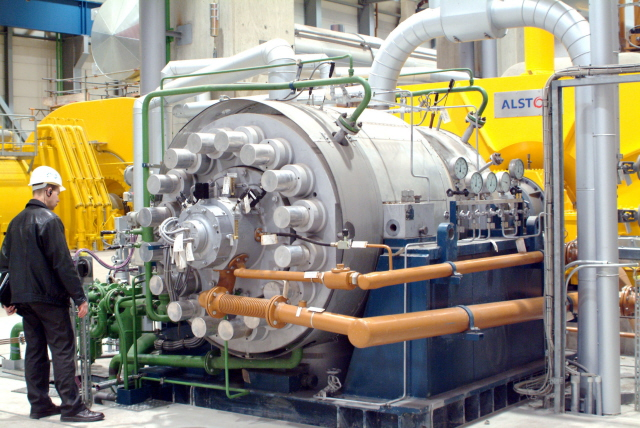
\includegraphics[height=8cm]{images/centrale_pompe_photo.jpg}
			\end{center}
			\supercaption{Photo d’une pompe du fabricant \textsc{ksb} menant \SI{2500}{\tonne\per\hour} d’eau à \SI{350}{\bar} dans une centrale à vapeur.\\
			Les pompes à liquide sont usuellement alimentées par un moteur électrique, mais ce modèle est alimenté mécaniquement par la turbine et doit ainsi fonctionner sur une plus grande plage de vitesses. Sa puissance maximale est de \SI{38}{\mega\watt} ; la puissance de la turbine entraînée dépasse \SI{800}{\mega\watt}.}{Photo \ccbysa \wcfile{Kesselspeisepumpe Kraftwerk Niederaussem.jpg}{KSB Aktiengesellschaft, Frankenthal}}
			\label{fig_centrale_pompe1}
		\end{figure}

		\begin{figure}
			\begin{center}
				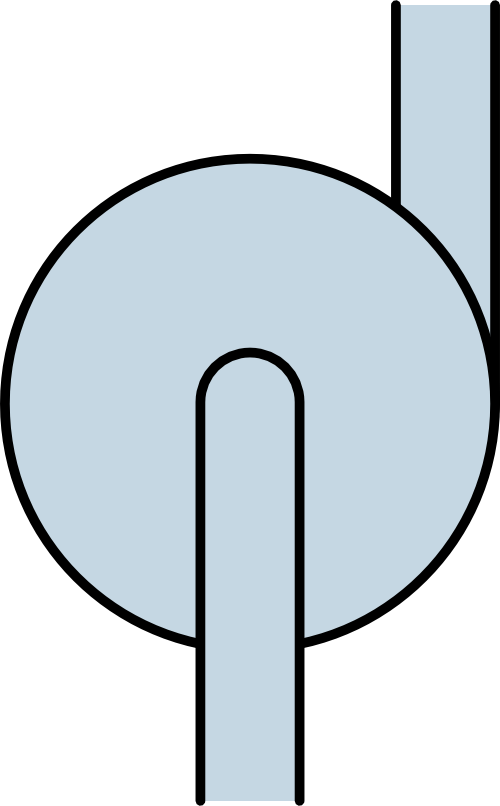
\includegraphics[height=4cm]{images/symbole_pompe.png}
			\end{center}
			\caption{Schéma de principe d’une pompe à eau.}
			\label{fig_centrale_pompe2}
		\end{figure}

		La puissance spécifique requise pour comprimer un débit de fluide d’une pression $p_A$ à une pression $p_B$, lorsque l’évolution est réversible, s’exprime à partir de la relation \ref{eq_travail_w_rév_so}. Comme le volume massique $v_L$  de l’eau liquide pure saturée (environ $v_L = \SI{1e-3}{\metre\cubed\per\kilogram}$) varie très peu avec sa pression, nous pouvons écrire :
		\begin{equation}
			w_\text{pompe~liquide} \approx v_L \int_\A^\B \diff p = v_L (p_\B - p_\A ) \label{eq_pompe_liquide}
		\end{equation}
		\begin{description}
			\item dans le cas d’une pompe approximativement réversible et fonctionnant avec de l’eau liquide.
		\end{description}

		 	\begin{anexample}
		 	\label{exemple_pompe_centrale}
		 		Dans une centrale, une pompe est alimentée par un débit de \SI{35}{\kilogram\per\second} d’eau liquide saturée à \SI{0,5}{\bar}. L’eau est comprimée de façon approximativement isentropique jusqu’à \SI{40}{\bar}. Quelle est la puissance consommée ?
		 			\begin{answer}
			 			L’évolution peut être représentée de façon qualitative sur un diagramme température-entropie ainsi :
						\begin{center}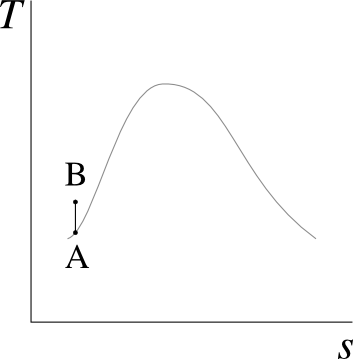
\includegraphics[width=4cm]{images/exe_ts_pompe.png}\end{center}
		 				Dans l’abaque~n°3 à \SI{0,05}{\mega\pascal} nous lisons l’enthalpie d’entrée $h_\A = h_{L \SI{0,05}{\mega\pascal}} = \SI{340,5}{\kilo\joule\per\kilogram}$. Le volume spécifique restera presque constant dans la pompe, à sa valeur de $v_\A = v_{L \SI{0,05}{\mega\pascal}} = \SI{0,00103}{\metre\cubed\per\kilogram}$. 
		 				
		 				Avec l’\cref{eq_pompe_liquide} nous calculons $\dot W_\text{pompe} \approx \dot m \ v_L (p_\B - p_\A ) = \num{35} \times \num{0,00103} (\num{40e5} - \num{0,5e5}) = \SI{+142,4}{\kilo\watt}$.
		 				
		 					\begin{remark}Comme la compression est par hypothèse isentropique, nous aurions aussi pu partir du fait que $s_\A = s_\B$ pour obtenir $h_\B$ par interpolation dans l’abaque~n°1 et calculer ainsi la puissance de la pompe. Un calcul de $v_\B$ avec cette méthode permet de se convaincre que le volume spécifique varie de manière imperceptible (moins de \SI{0,1}{\percent}) pendant cette évolution.\end{remark}
		 					\begin{remark}Comme nous avons calculé la puissance, nous sommes capables de calculer $h_\B = \frac{\dot W_\text{pompe}}{\dot m} + h_\A = \SI{482,9}{\kilo\joule\per\kilogram}$, c’est à dire l’enthalpie de l’eau à l’entrée de la chaudière, une  information très utile pour calculer sa puissance.\end{remark}
		 			\end{answer}
		 	\end{anexample}

	\subsection{Chaudière}
	\label{ch_chaudière}

		Dans les centrales à vapeur, les apports de chaleur se font à pression constante. L’eau du circuit thermodynamique est réchauffée par contact avec une autre canalisation : d’air dans le cas des centrales à combustion (déchets, charbon, gaz), ou d’eau (d’un circuit secondaire) dans le cas des centrales nucléaires%
		\footnote{Nous utilisons un deuxième circuit d’eau pour éviter de faire passer l’eau du circuit thermodynamique à haute pression dans le cœur même du réacteur.}\nolinebreak.

		L’extraordinaire comportement des fluides lorsqu’ils changent de phase tourne ici à notre avantage : en mélange di-phasique, une évolution à pression constante se fait aussi à température constante (\S\ref{ch_lv_diagramme_tv}),	ce qui nous permet de nous rapprocher des conditions prescrites par Carnot sans avoir recours à la moindre pièce mobile.
		
		Parce qu’elle fonctionne à haute pression (jusqu’à~\SI{60}{\bar} dans les installations modernes), et qu’elle est le théâtre de transferts de chaleur et gradients de température importants, la chaudière est un élément coûteux et lourd (figures~\ref{fig_centrale_chaudiere1} et~\ref{fig_centrale_chaudiere2}), même si son principe de fonctionnement est simple.

		\begin{figure}
			\begin{center}
				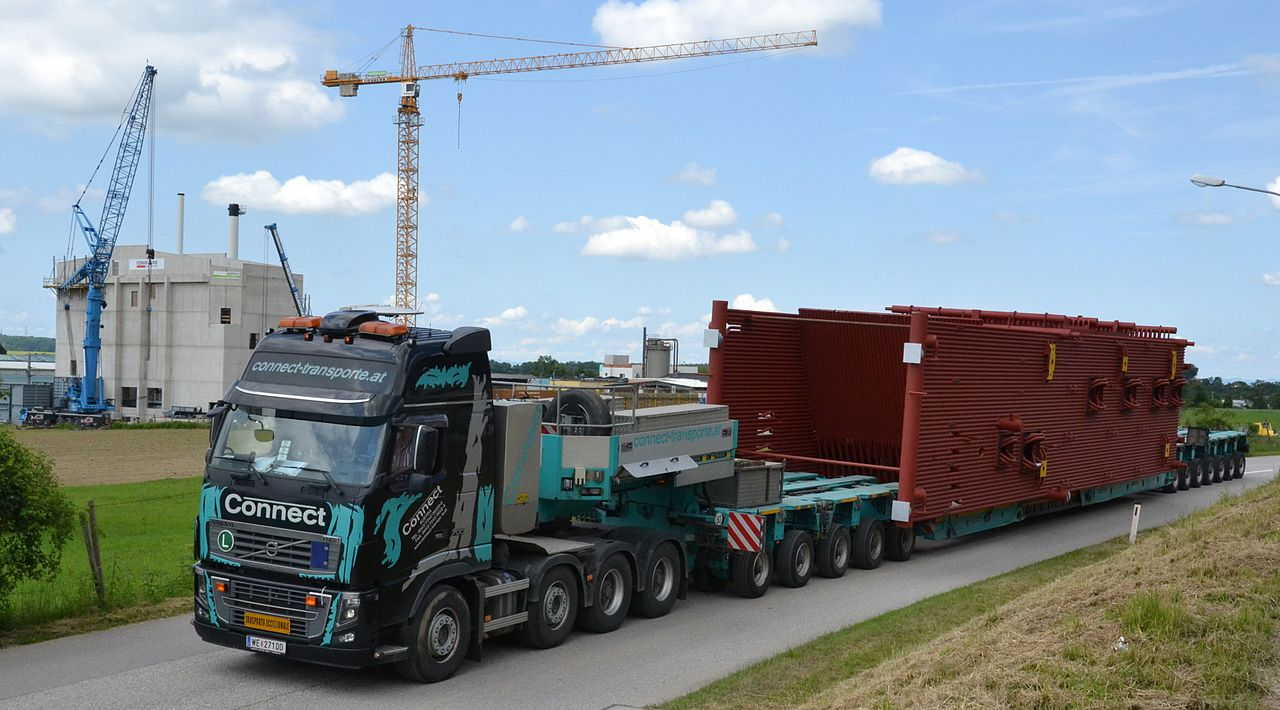
\includegraphics[width=\textwidth]{images/centrale_chaudiere_photo.jpg}
			\end{center}
			\supercaption{Transport d’une chaudière de centrale à bois capable de soutenir une pression de~\SI{100}{\bar}.}{\wcfile{Antransport_Flossenwandkessel_Steyr.jpg}{Photo} \ccbysa par \wcu{Sensenschmied}}
			\label{fig_centrale_chaudiere1}
		\end{figure}

		\begin{figure}
			\begin{center}
				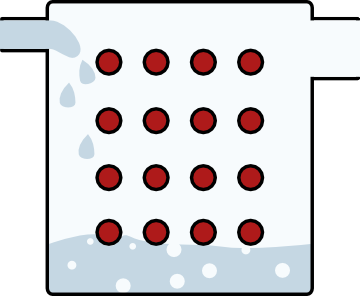
\includegraphics[width=4cm]{images/symbole_chaudiere.png}
			\end{center}
			\supercaption{Représentation schématique d’une chaudière.\\
		Dans une chaudière, l’eau pénètre à l’état liquide à gauche, et ressort en haut à droite à l’état de vapeur saturée. L’apport de chaleur est assuré par le contact avec les traverses des gaz de combustion.}{}
			\label{fig_centrale_chaudiere2}
		\end{figure}
		
		Lorsque la chaleur de la centrale provient d’une combustion, l’énergie thermique des gaz ne peut être transmise à l’eau du circuit que lorsque la température de cette dernière est plus faible. Ainsi, il est rejeté au-dessus de la chaudière une quantité de chaleur d’autant plus grande que la température minimale de l’eau y est haute. Le rendement $\eta_\text{chaudière} = \frac{\dot Q_\text{eau}}{\dot Q_\text{source de chaleur}}$ d’une chaudière à gaz performante avoisine usuellement les \SI{80}{\percent}.

		Comme aucun travail mécanique n’est fourni à l’eau dans la chaudière, la puissance $\dot{Q}_\text{chaudière}$ fournie par la chaudière à l’eau s’exprime selon :
		\begin{equation}
			\dot{Q}_\text{chaudière} = \dot{m} \ (h_2 - h_1)
		\end{equation}

		La différence de masse volumique entre les deux phases dans la chaudière fait qu’il est difficile de surchauffer la vapeur en présence de liquide (le liquide, plus dense et donc au fond de la chaudière, est en effet plus à même d’absorber la chaleur à haute température). Nous considérerons ainsi toujours que l’eau est sous forme de vapeur saturée (indice~$V$) à la sortie de la chaudière.


	\subsection{Turbine}

		La turbine (figures~\ref{fig_centrale_turbine1} et~\ref{fig_centrale_turbine2}) est la pièce maîtresse de toute centrale à vapeur. Longue de plusieurs dizaines de mètres dans les installations modernes, elle est équilibrée avec grand soin, mise en place dans son coffrage et, si elle fait l’objet d’attention adéquate (minimisation des gradients de température, lubrification avancée), peut délivrer de la puissance mécanique pendant plusieurs dizaines d’années sans aucune interruption.

		\begin{figure}
			\begin{center}
				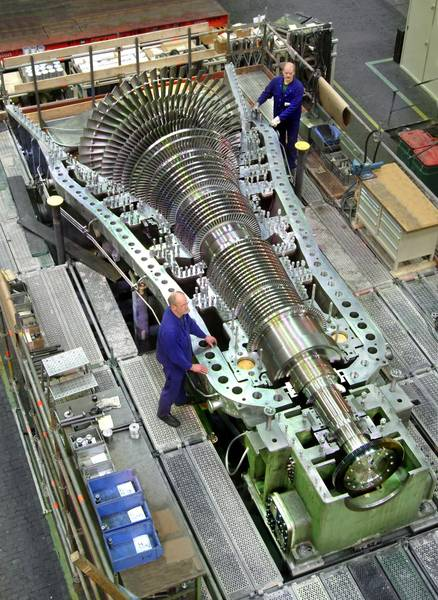
\includegraphics[height=9cm]{images/centrale_turbine_photo.jpg}
			\end{center}
			\supercaption{Turbine d’une centrale à vapeur de taille moyenne.\\
			Au fur et à mesure que l’eau traverse la turbine, elle perd de l’énergie sous forme de travail et son volume spécifique augmente, ce qui nécessite des pales toujours plus grandes.}{\wcfile{SteamTurbine.jpg}{Photo} \ccbysa MAN SE}
			\label{fig_centrale_turbine1}
		\end{figure}

		\begin{figure}
			\begin{center}
				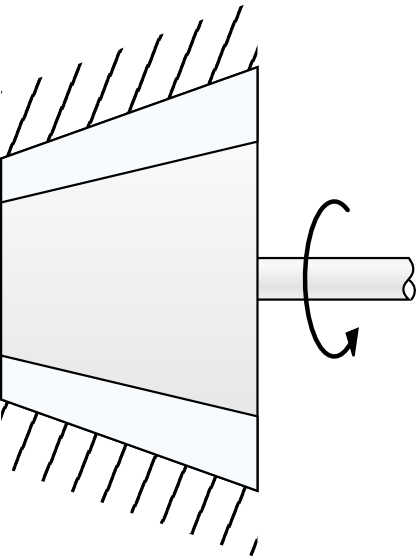
\includegraphics[width=4cm]{images/symbole_turbine.png}
			\end{center}
			\caption{Représentation schématique d’une turbine à vapeur.}
			\label{fig_centrale_turbine2}
		\end{figure}
		

		L’efficacité d’une turbine se mesure en comparant sa puissance avec celle d’une turbine idéale (une turbine qui serait isentropique). Nous nommons ce paramètre l’\vocab{efficacité isentropique} :
		\begin{equation}
			\eta_\text{T} \equiv  \frac{\dot{W}_\text{turbine réelle}}{\dot{W}_\text{turbine isentropique}}
			\label{def_efficacité_isentropique_turbine}
		\end{equation}
		
		\begin{equationterms}
			\item pour une turbine,
			\item où \tab $\dot{W}_\text{turbine réelle}$ 			\tab\tab\tab\tab\tab est la puissance réelle fournie par la turbine,
			\item et \tab $\dot{W}_\text{turbine isentropique}$ 	\tab la puissance d’une turbine isentropique fonctionnant avec le même débit de masse et entre les deux mêmes pressions.
		\end{equationterms}

		La puissance réelle, quant à elle, s’exprime toujours en fonction des propriétés du fluide à l’entrée et à la sortie de la turbine :
		\begin{equation}
			\dot{W}_\text{turbine réelle} = \dot{m} \ (h_{2 \text{réel}} - h_1) = \dot m \ \eta_\text{T} \ (h_{2’} - h_1)
			\label{eq_puissance_turbine_vapeur}
		\end{equation}

		Avec une combinaison des équations~\ref{def_efficacité_isentropique_turbine} et~\ref{eq_puissance_turbine_vapeur}, on peut ainsi prévoir l’état de la vapeur à la sortie de n’importe quelle turbine dont on connaît la puissance et l’efficacité isentropique.

		Un paramètre important qui doit être surveillé est le titre de l’eau, en particulier dans les derniers étages. Les gouttelettes liquides, beaucoup plus denses que la vapeur qui les entoure, percutent en effet violemment les pales et en provoquent l’érosion. L’ingénieur/e thermodynamicien/ne veillera ainsi à garder un haut titre, usuellement sans descendre en deçà de~\SI{95}{\percent}.

		\begin{anexample}
		\label{exemple_turbine_centrale}
			Une turbine d’efficacité isentropique \SI{85}{\percent} reçoit \SI{35}{\kilogram\per\second} d’eau à \SI{40}{\bar} et \SI{600}{\degreeCelsius}. Elle détend l’eau jusqu’à \SI{0,5}{\bar}. Quelle est la puissance développée ?
				\begin{answer}
					L’évolution peut être représentée de façon qualitative sur un diagramme température-entropie ainsi :
						\begin{center}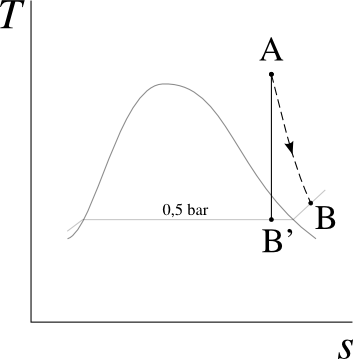
\includegraphics[width=4cm]{images/exe_ts_turbine.png}\end{center}
					Nous commençons par imaginer que nous sommes dotés --\ irrépressible fantasme de thermodynamicien/ne !-- d’une turbine isentropique entre ces deux mêmes pressions. Dans l’abaque~n°1 à \SI{4}{\mega\pascal}, nous lisons $h_\A = \SI{3674,9}{\kilo\joule\per\kilogram}$ et $s_\A = \SI{7,3705}{\kilo\joule\per\kelvin\per\kilogram}$. La vapeur à la sortie de cette turbine hypothétique (en B’) a la même entropie : $s_{\B’} = s_\A$, et nous constatons que $s_{\B’} < s_{V \SI{0,05}{\mega\pascal}}$ : l’eau est partiellement condensée. Le calcul du titre (\S\ref{ch_melange_liquide_vapeur}) nous permet de calculer la valeur de son enthalpie : $h_{\B’} = h_{L \SI{0,05}{\mega\pascal}} + \frac{s_{\B’} - s_{L \SI{0,05}{\mega\pascal}}}{s_{LV \SI{0,05}{\mega\pascal}}} h_{LV \SI{0,05}{\mega\pascal}} = \SI{2566,3}{\kilo\joule\per\kilogram}$.
					
					Le retour à la réalité est douloureux : la turbine réelle ne développe que \SI{85}{\percent} de la puissance de cette turbine hypothétique, ainsi $\dot{W}_\text{turbine réelle} = \dot{m} \ \eta_\text{T} \ (h_{\B’} - h_\A) = \num{35} \times \num{0,85} \times (\num{2566,3e3} - \num{3674,9e3}) = \SI{-32 980}{\kilo\watt} = \SI{-32,98}{\mega\watt}$.
						\begin{remark}L’\cref{eq_puissance_turbine_vapeur} nous permet de calculer l’enthalpie $h_\B$ réellement obtenue la sortie de la turbine : $h_\B = \frac{\dot W_\text{turbine}}{\dot m} + h_\A = \SI{2732,6}{\kilo\joule\per\kilogram}$, ce qui est très utile pour calculer ensuite la puissance du condenseur. Un coup d’œil à l’abaque~n°2 nous montre que $h_\B > h_{V \SI{0,05}{\mega\pascal}}$ : la vapeur est donc sèche tout le long de sa détente.\end{remark}
						\begin{remark}Les \SI{15}{\percent} de puissance manquants dans l’arbre mécanique de la turbine sont transférés sous forme de chaleur et turbulence à l’eau pendant sa détente dans la turbine.\end{remark}
						\begin{remark}La puissance de la turbine est deux-cent fois plus importante (!) que la puissance consommée par la pompe de l’exemple~\ref{exemple_pompe_centrale} entre ces deux mêmes pressions.\end{remark}
				\end{answer}
		\end{anexample}

	\subsection{Condenseur}

		Le condenseur (figures~\ref{fig_centrale_condenseur1} et~\ref{fig_centrale_condenseur2}), composant le moins glorieux de l’installation, est en charge de rejeter toute la chaleur dont l’ingénieur/e ne sait plus faire usage (\S\ref{ch_second_principe_machines_thermiques}). L’eau y est toujours refroidie à pression constante, ce qui ne nécessite pas de pièce mobile.

		\begin{figure}
			\begin{center}
				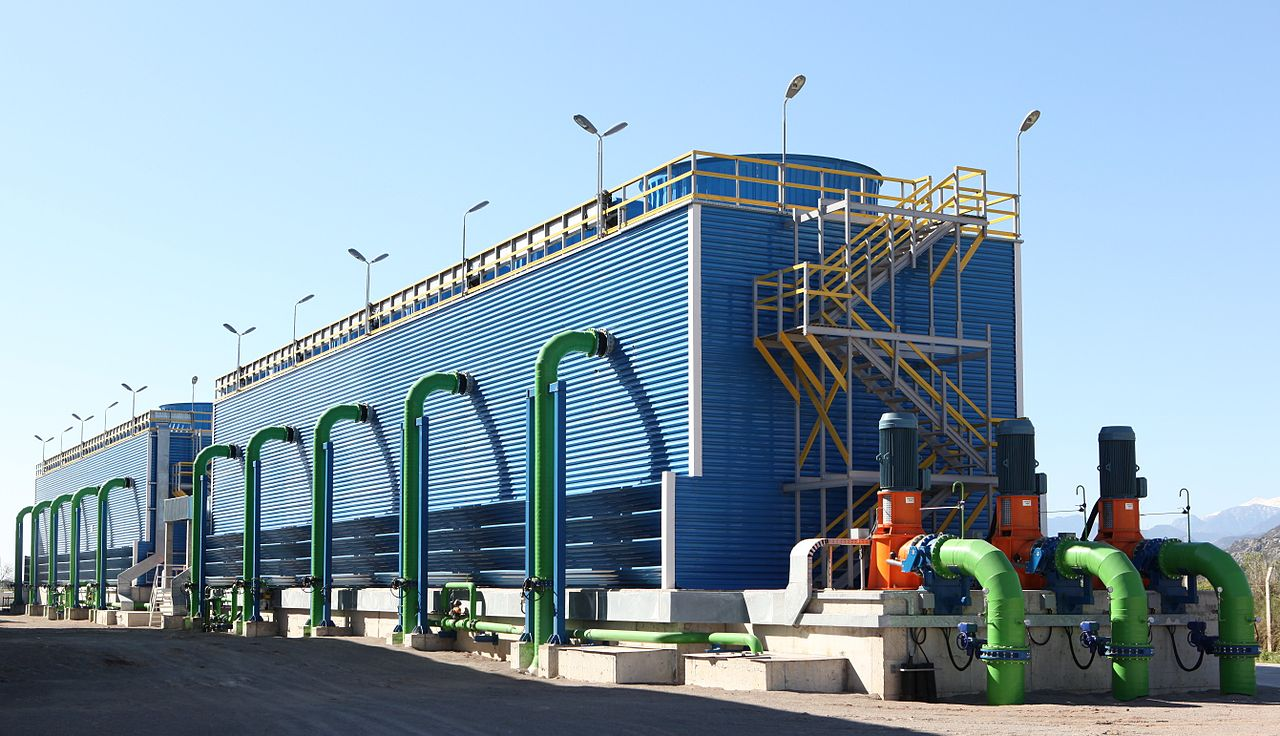
\includegraphics[width=\textwidth]{images/centrale_condenseur_photo.jpg}
			\end{center}
			\supercaption{Un condenseur dans lequel la chaleur est évacuée directement dans l’atmosphère, par conduction forcée à l’aide de ventilateurs.}{\wcfile{Cenk_Endustri_Field_Erected_Industrial_Cooling_Tower.JPG}{Photo} \ccbysa Cenk Endustri}
			\label{fig_centrale_condenseur1}
		\end{figure}

		\begin{figure}
			\begin{center}
				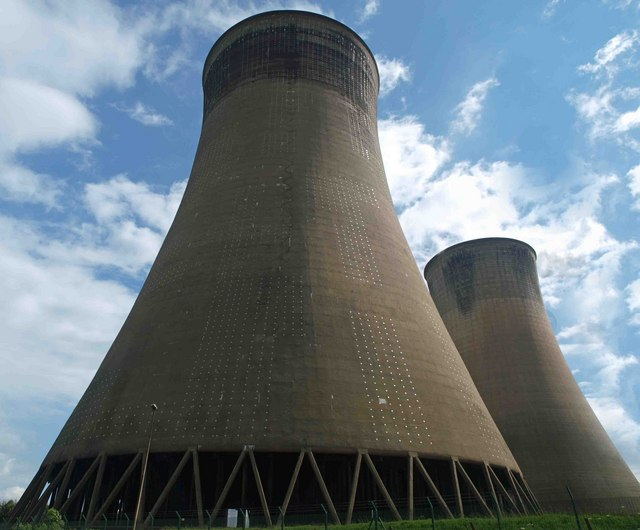
\includegraphics[width=0.7\textwidth]{images/cooling_towers.jpg}
			\end{center}
			\supercaption{Cheminées de refroidissement de la centrale à charbon de Eggborough (1967, \SI{1960}{\giga\watt}) au Royaume-Uni. Dans ces cheminées, la chaleur prélevée à l’eau du circuit dans le condenseur est évacuée dans l’atmosphère. Ce refroidissement est effectué au moyen d’un circuit d’eau secondaire, qui est mis en contact avec l’atmosphère et s’y évapore partiellement.}{\wcfile{Eggborough cooling towers ^1 - geograph.org.uk - 844420.jpg}{Photo} \ccbysa \href{http://www.geograph.org.uk/profile/15341}{Steve Fareham}}
			\label{fig_centrale_condenseur1}
		\end{figure}

		\begin{figure}
			\begin{center}
				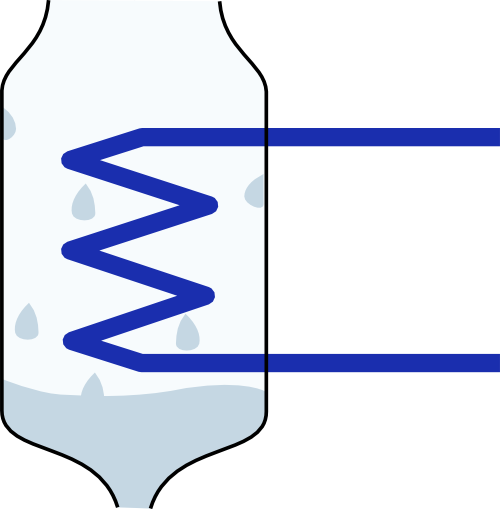
\includegraphics[width=4cm]{images/symbole_condenseur.png}
			\end{center}
			\supercaption{Représentation schématique d’un condenseur.\\
			L’eau du circuit thermodynamique y pénètre par le haut, dans un état proche de la vapeur saturée. Elle en ressort par le bas à l’état liquide. L’extraction de chaleur est usuellement assurée par un circuit d’eau secondaire (schématisé en bleu) qui elle est mise en contact avec l’atmosphère.}{}
			\label{fig_centrale_condenseur2}
		\end{figure}

		Technologiquement, le condenseur est un élément simple : on met simplement la canalisation de vapeur en contact avec un circuit de température basse. Usuellement, ce circuit de refroidissement est constitué d’eau extérieure provenant d’une rivière ou de la mer,\footnote{Il y a deux intérêts à l’utilisation d’un circuit de refroidissement secondaire. D’une part, on peut abaisser la pression dans le condenseur plus bas que la pression atmosphérique et ainsi réduire la température minimale du cycle. D’autre part, l’eau du circuit thermodynamique, épurée au prix d’efforts considérables, n’est pas perdue dans l’atmosphère.}
		qui sera refroidie ensuite par évaporation dans les larges cheminées que l’on aperçoit aux abords des centrales. Comme la pression de la vapeur à l’intérieur du condenseur est souvent très basse (jusqu’à~\SI{0,1}{\bar}) pour abaisser la température minimale du cycle de la centrale, il faut veiller à l’étanchéité du condenseur pour éviter que de l’air ou de l’eau extérieurs ne s’insèrent dans le circuit principal.

		La puissance perdue par la vapeur dans le condenseur s’exprime selon :
		\begin{equation}
			\dot{Q}_\text{condenseur} = \dot{m} \ (h_2 - h_1)
		\end{equation}



\section{Cycles moteurs à vapeur}

	\subsection{Le cycle de Carnot}

		Comme le cycle de Carnot que nous avons étudié au \S\ref{ch_cycle_de_carnot} nous sert de référence dans la conception des moteurs, nous débutons notre étude par celui-ci. La température d’un mélange liquide-vapeur reste constante lorsqu’on le chauffe à pression constante, aussi la réalisation d’échanges de chaleur isotherme (caractéristique importante du cycle de Carnot) est relativement aisée avec la vapeur. Une machine à vapeur basée sur un cycle de Carnot est schématisée en figures~\ref{fig_machine_vapeur_carnot} et~\ref{fig_ts_machine_vapeur_carnot}.

		\begin{figure}
			\begin{center}
				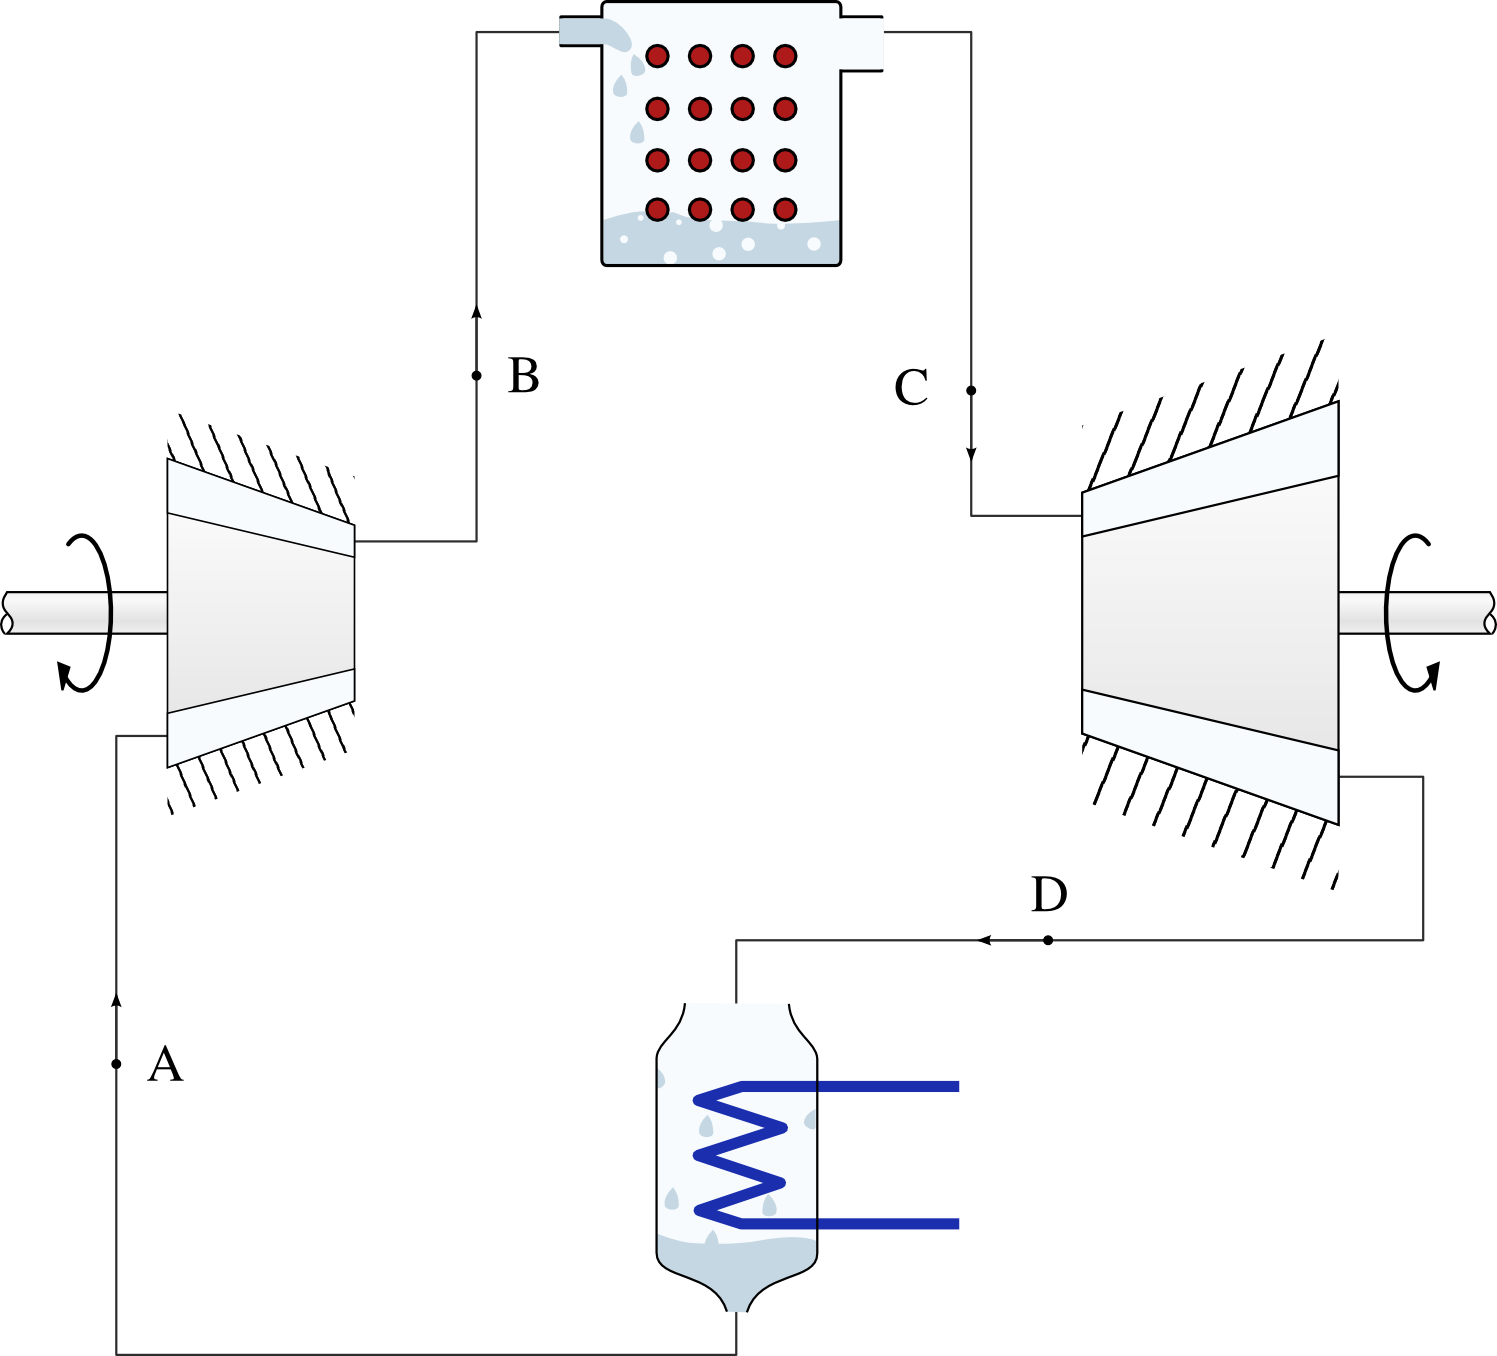
\includegraphics[height=11cm]{images/circuit_carnot_lv.png}
			\end{center}
			\supercaption{Circuit d’une centrale à vapeur fonctionnant sur un cycle de Carnot.}{schéma \ccbysa \olivier}
			\label{fig_machine_vapeur_carnot}
		\end{figure}

		\begin{figure}
			\begin{center}
				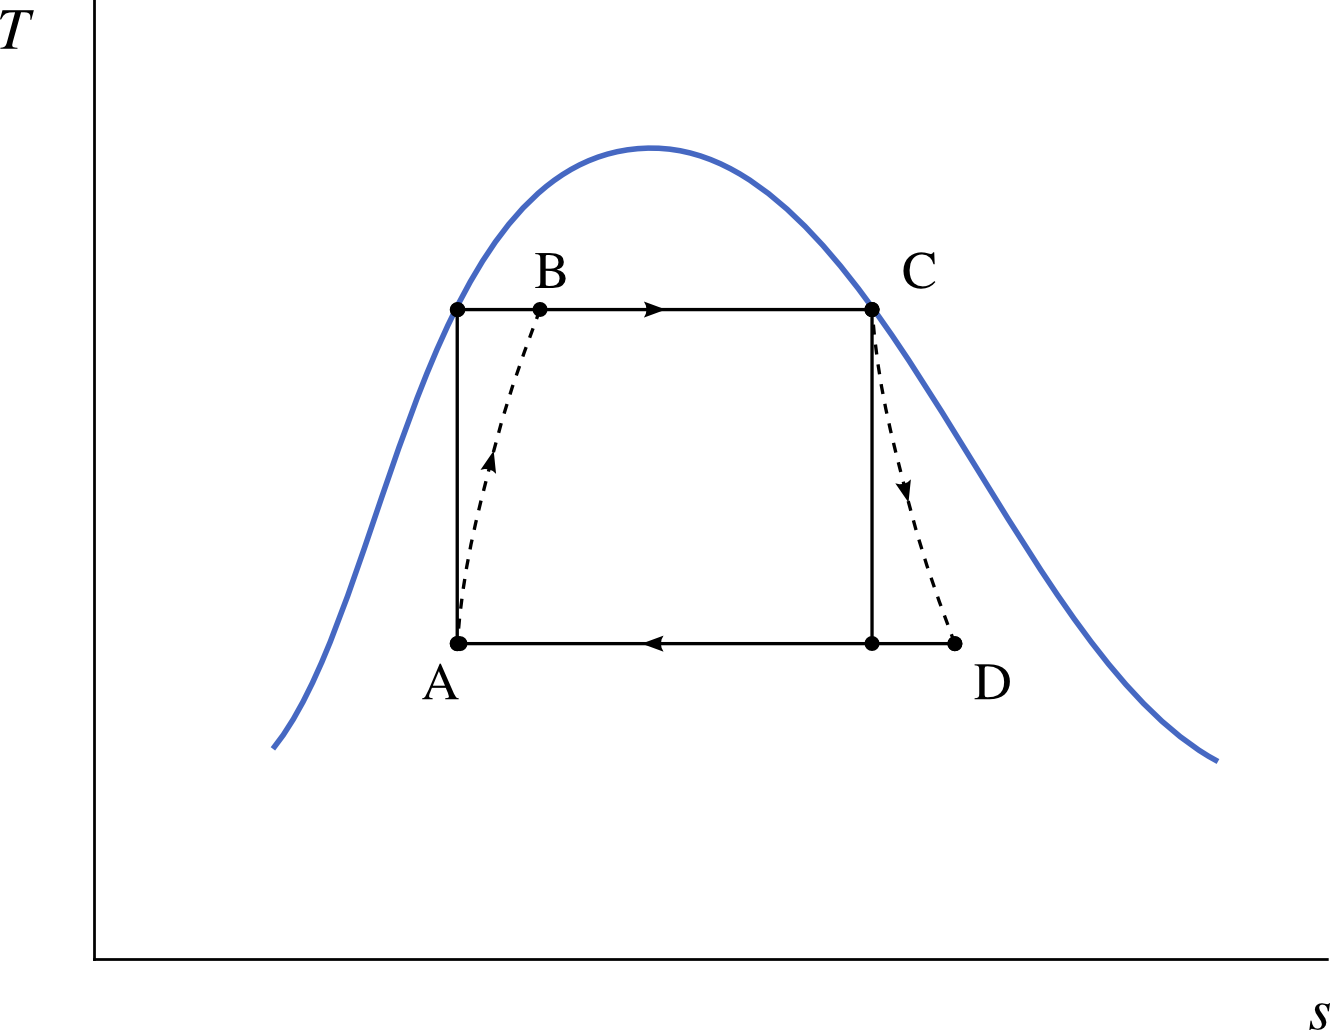
\includegraphics[width=10cm]{images/ts_lv_carnot.png}
			\end{center}
			\supercaption{Diagramme température-entropie d’une centrale à vapeur fonctionnant sur un cycle de Carnot. Les trajets en pointillés représentent les évolutions réelles (irréversibles) du fluide pendant les compressions et détentes.}{schéma \cczero \oc}
			\label{fig_ts_machine_vapeur_carnot}
		\end{figure}

		L’efficacité du cycle moteur de Carnot (\ref{eq_efficacité_moteur_carnot_température}) n’est atteinte que lorsque la turbine et le compresseur fonctionnent de façon isentropique. En pratique, comme nous l’avons vu, la puissance de la turbine est toujours plus faible et celle du compresseur toujours plus grande qu’elles ne pourraient l’être.


	\subsection{Le cycle de Rankine}
	\label{ch_cycle_de_rankine}

		En pratique, l’utilisation du cycle de Carnot comme ci-haut pose plusieurs difficultés :

		\begin{itemize}
			\item La compression d’un mélange di-phasique est technologiquement difficile (\S\ref{ch_moteurs_vapeur_compresseurs_et_pompes}) ;
			\item Dans le condenseur, il est difficile d’interrompre la condensation à un endroit précis (le point A en figures~\ref{fig_machine_vapeur_carnot} et~\ref{fig_ts_machine_vapeur_carnot} plus haut, dont le titre est proche mais différent de~0).
		\end{itemize}

		\wed{William John Macquorn Rankine}{William Rankine}, ingénieur anglo-saxon digne de ses compatriotes, propose en 1859 une modification du cycle en poursuivant la condensation jusqu’à saturation et en ne compressant l’eau qu’à l’état liquide. Une machine basée sur ce cyle est décrite en figures~\ref{fig_cycle_rankine} et~\ref{fig_ts_lv_rankine}.

		\begin{figure}
			\begin{center}
				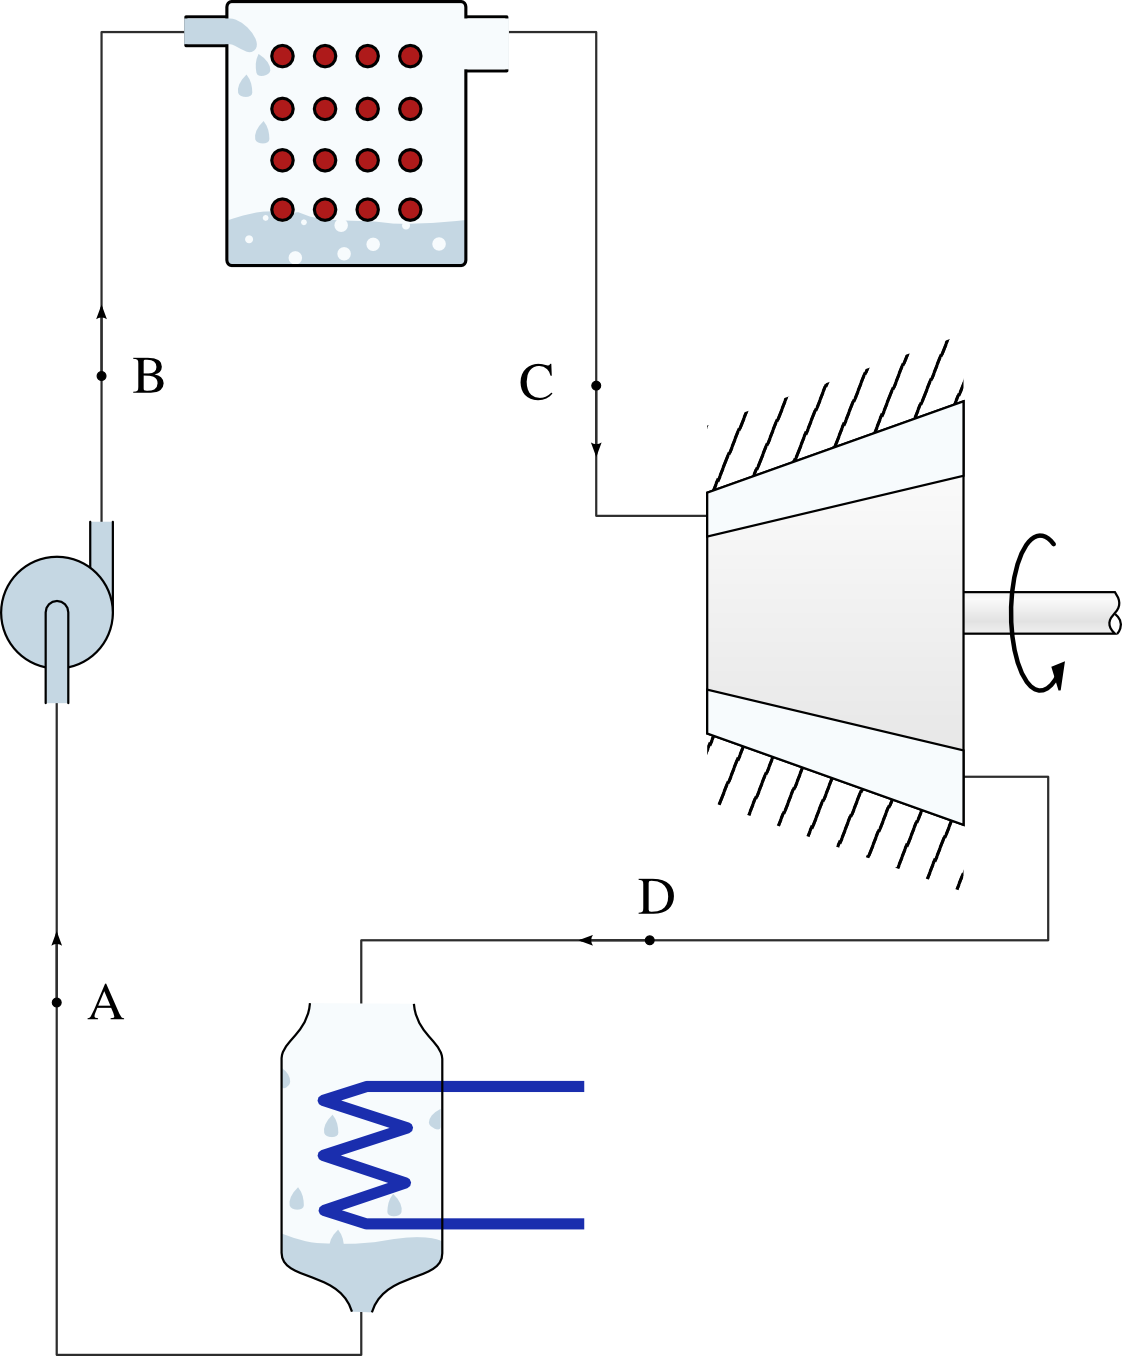
\includegraphics[height=11cm]{images/circuit_rankine.png}
			\end{center}
			\supercaption{Circuit d’une centrale à vapeur fonctionnant sur un cycle de Rankine. L’eau à la sortie du condenseur est sous forme de liquide saturée ; elle rentre dans la chaudière à plus faible température.}{schéma \ccbysa \olivier}
			\label{fig_cycle_rankine}
		\end{figure}

		\begin{figure}
			\begin{center}
				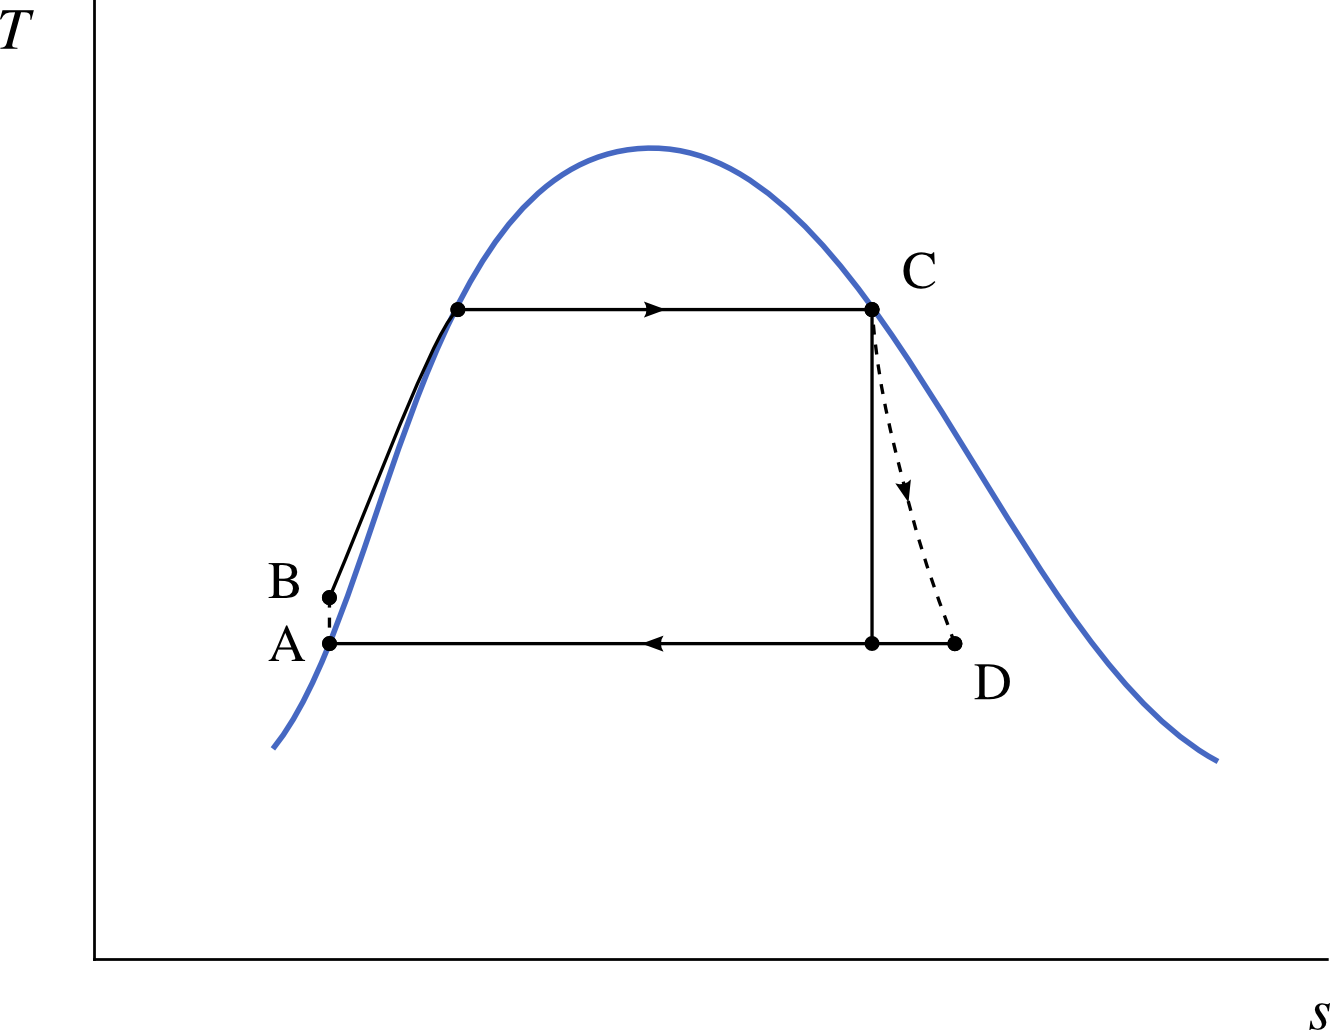
\includegraphics[width=10cm]{images/ts_lv_rankine.png}
			\end{center}
			\supercaption{Diagramme température-entropie d’une centrale à vapeur fonctionnant sur un cycle de Rankine.}{schéma \cczero \olivier}
			\label{fig_ts_lv_rankine}
		\end{figure}

		Le \vocab{cycle de Rankine} utilise donc une pompe à eau liquide plutôt qu’un compresseur en mélange liquide/vapeur. Technologiquement, une pompe est plus simple à concevoir, fabriquer, et opérer qu’un compresseur. Autre avantage, la compression d’un liquide est plusieurs dizaines de fois plus économe en énergie que celle du mélange (\S\ref{ch_moteurs_vapeur_compresseurs_et_pompes}). 
		
		Toutefois, cette économie d’énergie n’est pas sans contrepartie : à la sortie de la pompe (point B), l’eau est à température bien plus faible qu’elle ne l’était à la sortie du compresseur en \cref{fig_machine_vapeur_carnot}. C’est \emph{la chaudière} qui devra ramener l’eau à l’état de liquide saturé. Autrement dit, il faut fournir une dépense supplémentaire considérable sous forme de chaleur pour compenser la baisse de puissance de compression.

		On peut remarquer qu’une partie importante de la chaleur fournie par la chaudière (c’est-à-dire $q_\text{chaudière} = h_\C - h_B$ ) n’est plus apportée à la température maximale du cycle. Nous avons vu aux chapitres~\sept et~\huit qu’un apport de chaleur à basse température se traduit toujours par un rendement plus faible.\\
		Toutefois, en pratique, cet apport de chaleur peut rendre possible l’exploitation de sources de chaleur à basse température, comme les gaz d’échappement qui étaient auparavant rejetés au-dessus de la chaudière. Ainsi, dans certains cas, la chute du rendement thermodynamique ($\eta_\text{moteur}$) peut être compensée par une augmentation du rendement de la chaudière ($\eta_\text{chaudière}$), qui peut extraire plus d’énergie au combustible pour le transmettre à la vapeur.
		
		Rankine s’est ainsi écarté volontairement du cycle de Carnot, et a ce faisant réduit le rendement thermodynamique global (même si cette baisse peut souvent être compensée par une augmentation du rendement de la chaudière). Par contre, en faisant disparaître le compresseur, sa modification permet de réduire fortement la taille et la complexité de l’installation.

		 

	\subsection{La surchauffe}

		Pour réduire la consommation spécifique ($SSC$) d’une centrale, il est souhaitable d’augmenter la puissance développée par la turbine pour un débit de vapeur donné. Pour cela, il existe plusieurs options :

		\begin{itemize}
			\item Augmenter l’enthalpie à l’entrée de la turbine (c’est-à-dire augmenter la pression de saturation dans la chaudière). \\
			Malheureusement, cela impose à la chaudière d’être plus résistante et plus coûteuse ; et de plus, cela réduit la quantité de chaleur spécifique qu’il est possible d’y apporter, puisque l’enthalpie de vaporisation $h_{LV}$ décroît avec la température ;

			\item Réduire l’enthalpie à la sortie de la turbine (c’est-à-dire diminuer la pression dans le condenseur). \\
			Cela nécessite une turbine de plus grande taille,  favorise l’insertion de bulles d’air dans le circuit de vapeur, et surtout, réduit le titre de l’eau en sortie de turbine ;

			\item Augmenter l’enthalpie (et donc la température de la vapeur) \emph{après} sa sortie de la chaudière.\\
			Cela permet  d’utiliser pleinement les capacités de la turbine, dont les limites métallurgiques (généralement autour de~\SI{1000}{\kelvin}) dépassent déjà souvent celles des chaudières.
		\end{itemize}

		C’est cette dernière option qui est très souvent choisie. On nomme cette modification la \vocab{surchauffe} : la vapeur est surchauffée à la sortie de la chaudière%
		\footnote{La surchauffe pourrait théoriquement être effectuée dans la chaudière même ; cependant, la densité de la vapeur surchauffée étant relativement faible, il est plus aisé de la mettre en contact avec les gaz les plus chauds en dehors (et en dessous) de la chaudière.}, à pression constante, à travers une série de tubes portés à plus haute température (figures~\ref{fig_cycle_rankine_surchauffe} et~\ref{fig_ts_lv_rankine_surchauffe}).

		\begin{figure}
			\begin{center}
				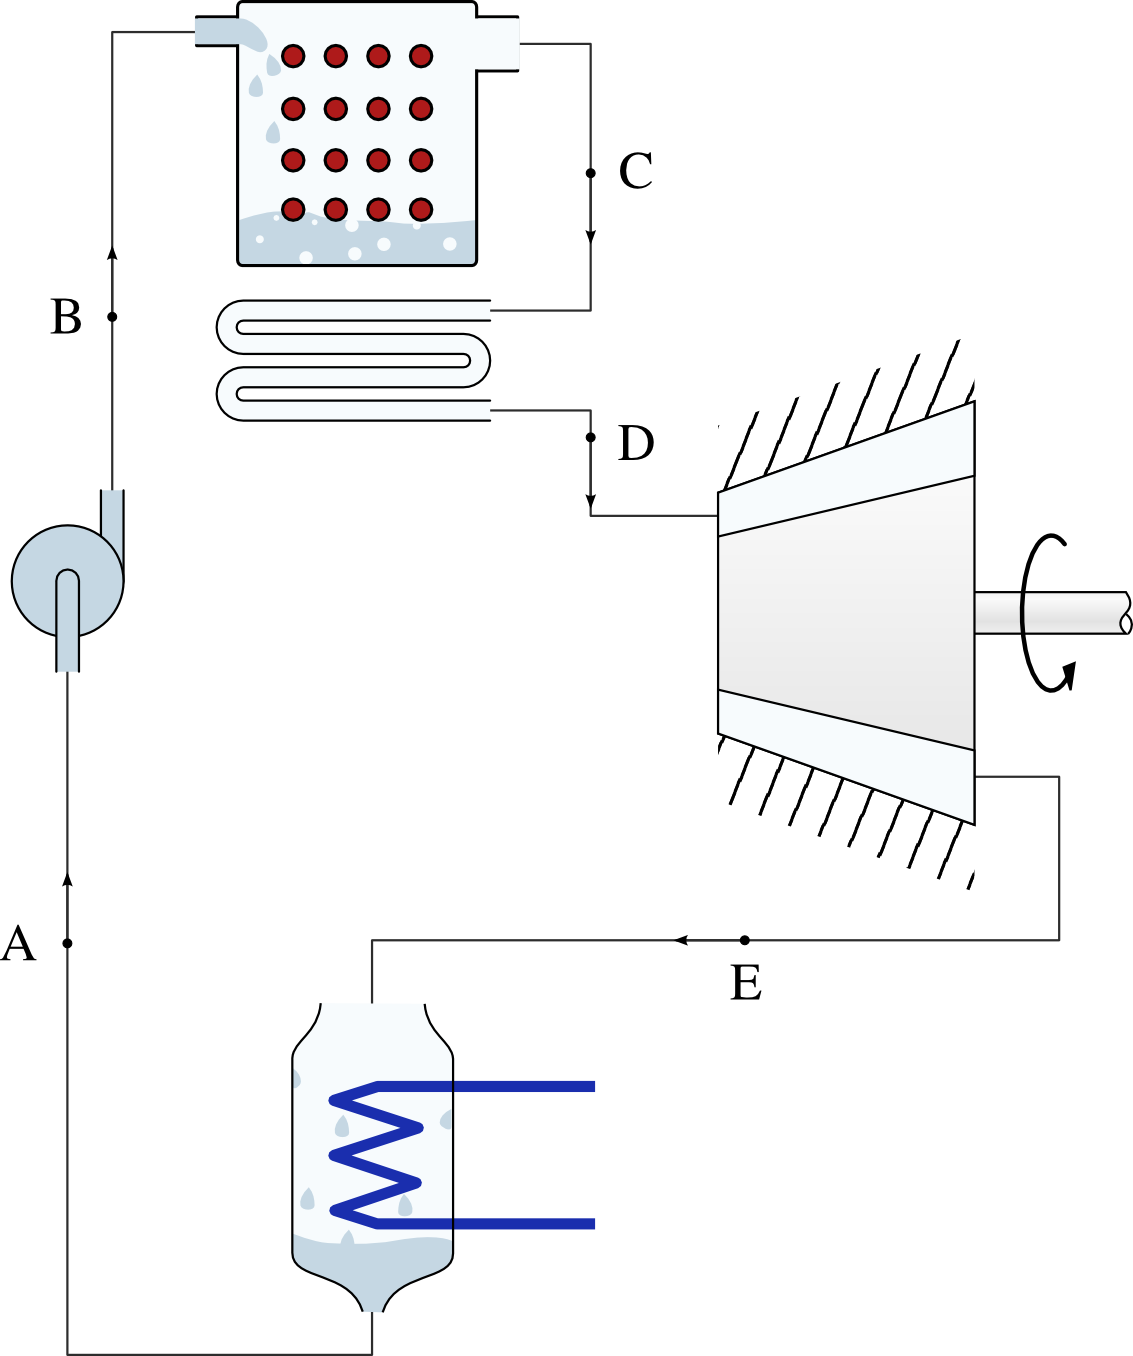
\includegraphics[height=11cm]{images/circuit_rankine_surchauffe.png}
			\end{center}
			\supercaption{Circuit d’une centrale à vapeur fonctionnant sur un cycle de Rankine surchauffé. L’eau à la sortie de la chaudière est portée à plus haute température (section C $\rightarrow $ D) avant de pénétrer dans la turbine.}{schéma \ccbysa \olivier}
			\label{fig_cycle_rankine_surchauffe}
		\end{figure}

		\begin{figure}
			\begin{center}
				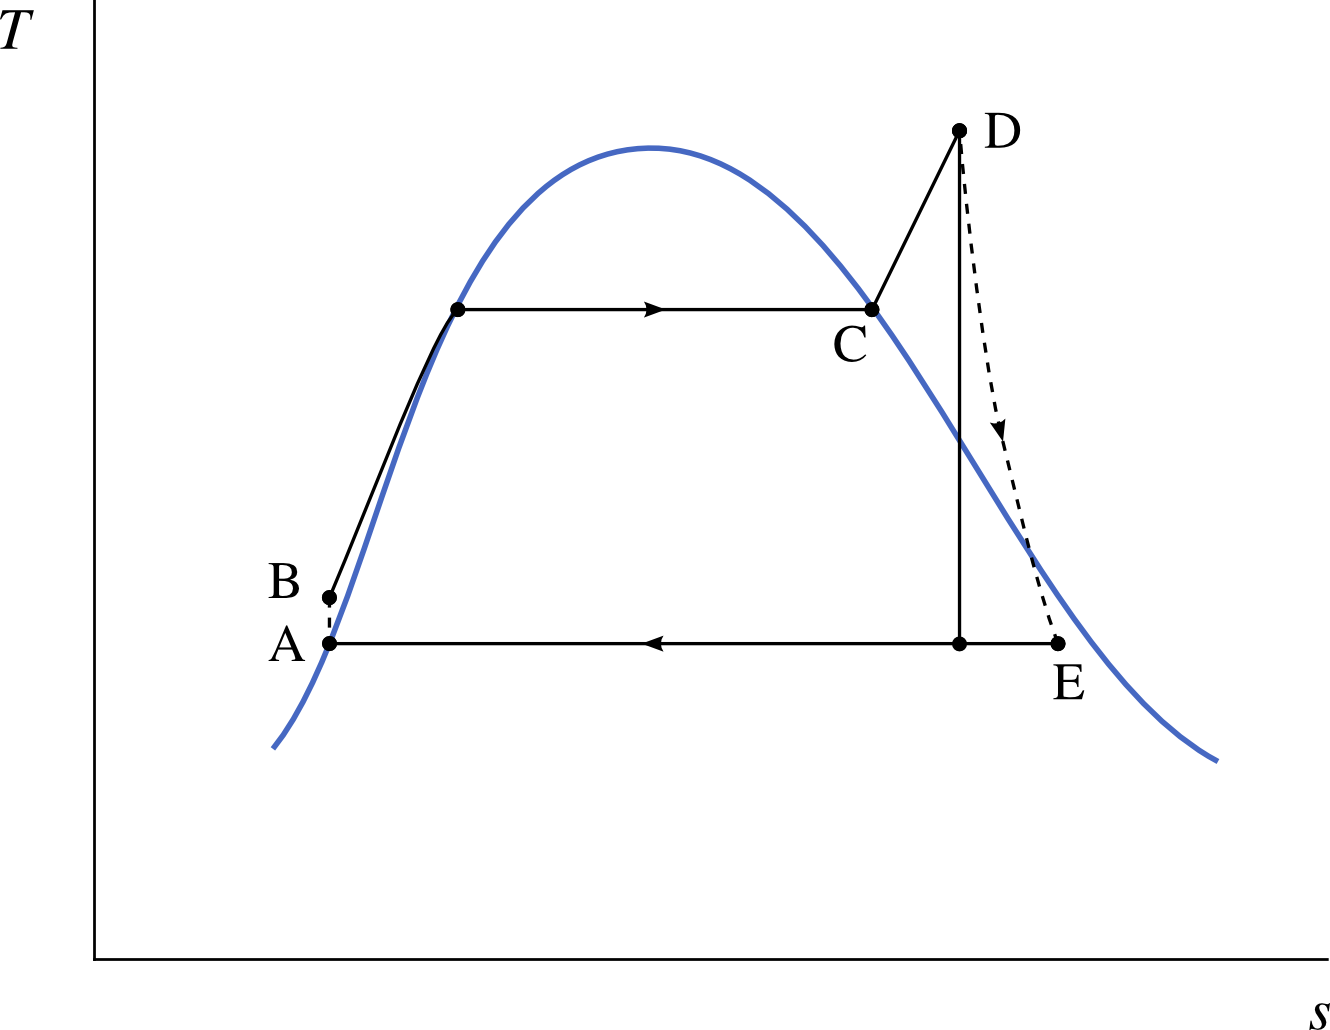
\includegraphics[width=10cm]{images/ts_lv_rankine_surchauffe.png}
			\end{center}
			\supercaption{Diagramme température-entropie d’une centrale à vapeur fonctionnant sur un cycle de Rankine surchauffé.}{schéma \cczero \oc}
			\label{fig_ts_lv_rankine_surchauffe}
		\end{figure}

		L’avantage principal de cette modification est qu’elle permet une diminution de la consommation spécifique peu complexe à mettre en œuvre. Autre avantage, l’augmentation de la température moyenne à laquelle la chaleur est apportée tend à augmenter le rendement thermodynamique. Enfin, il devient possible de décaler la plage d’utilisation de la turbine entièrement dans le domaine de la vapeur surchauffée : l’érosion des pales par l’eau liquide est ainsi évitée. De fait, toutes les installations à vapeur modernes utilisent un circuit de surchauffe.


	\subsection{La resurchauffe}
	\label{ch_resurchauffe}

		Pour augmenter à nouveau la puissance de l’installation sans augmenter le débit de vapeur (et donc sa taille globale et le coût de la chaudière), il est possible de chauffer une deuxième fois la vapeur avant sa sortie de la turbine (figures~\ref{fig_cycle_resurchauffe} et~\ref{fig_ts_lv_surchauffe_resurchauffe}). C’est ce que l’on appelle la \vocab{resurchauffe}.

		\begin{figure}
			\begin{center}
				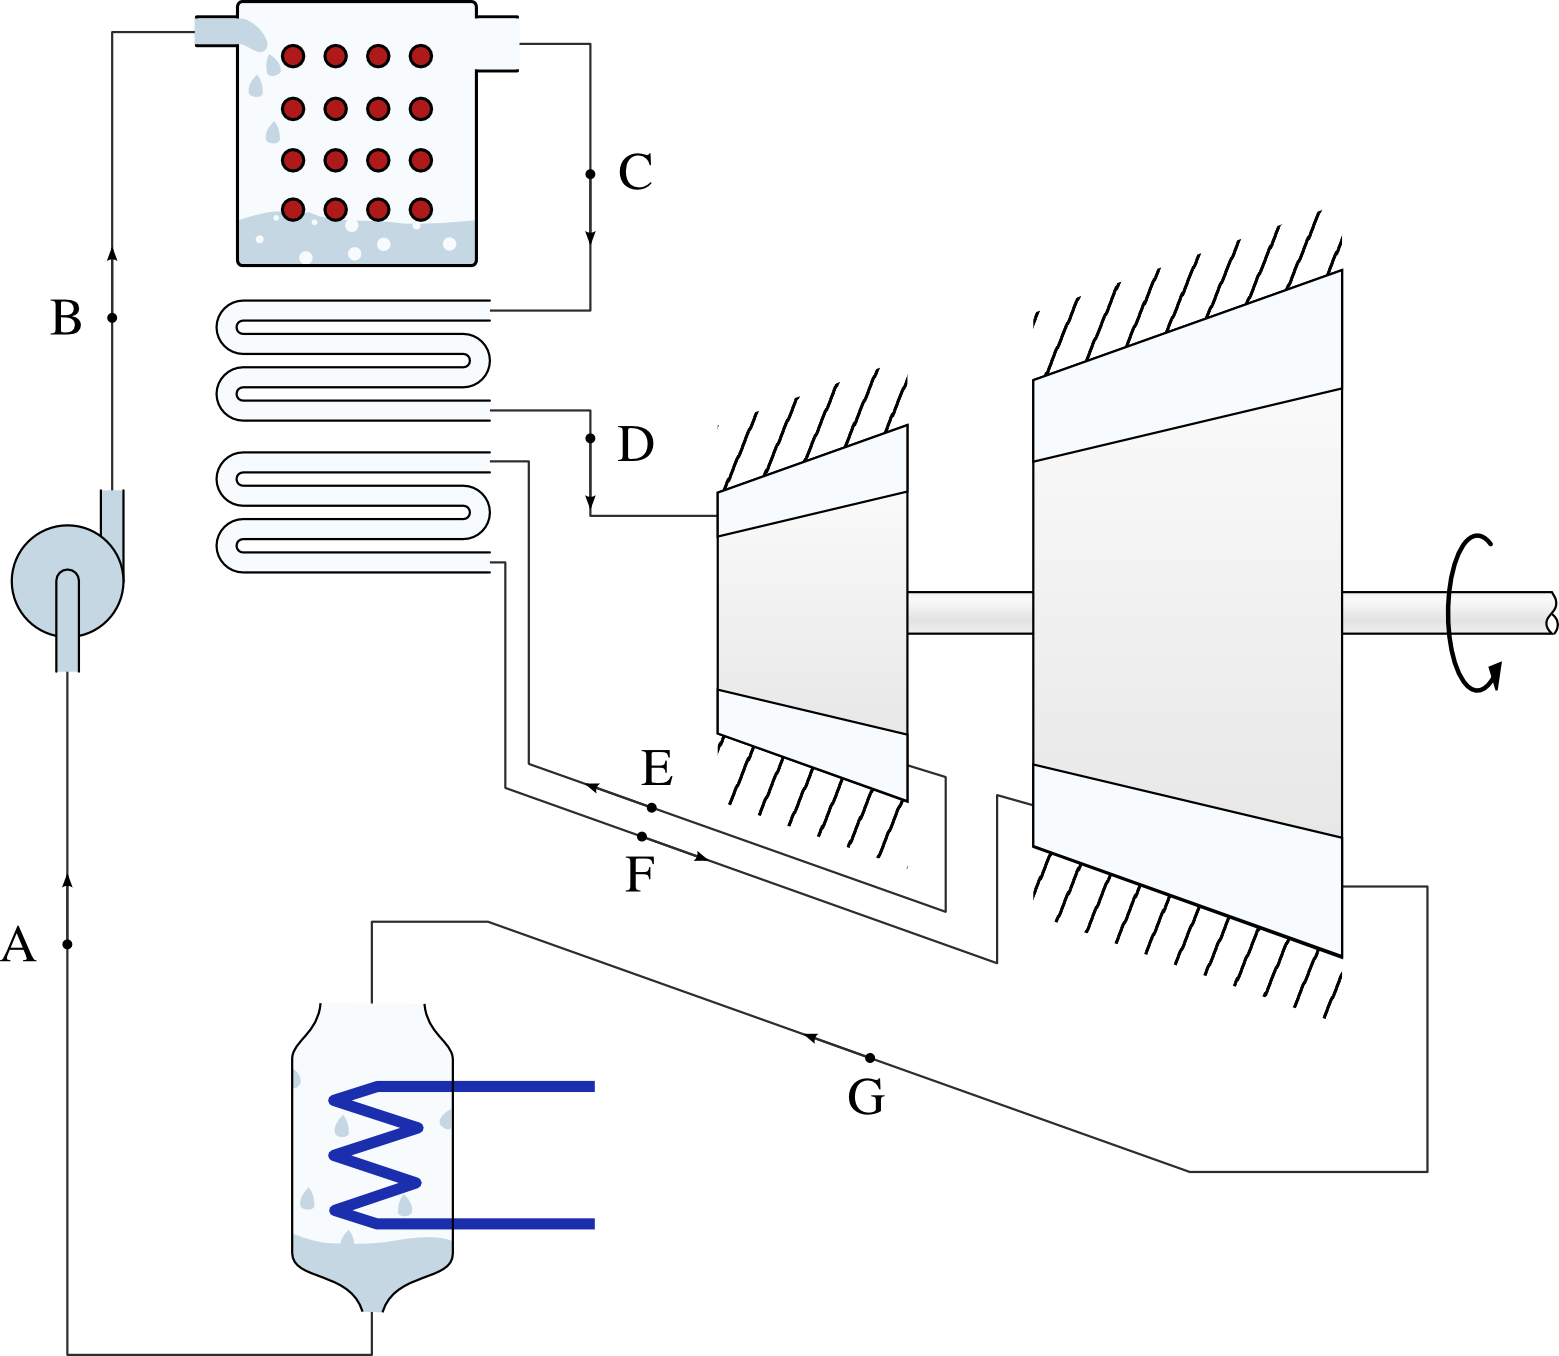
\includegraphics[height=11cm]{images/circuit_surchauffe_resurchauffe.png}
			\end{center}
			\supercaption{Circuit d’une centrale à vapeur fonctionnant sur un cycle de Rankine resurchauffé.}{schéma \ccbysa \olivier}
			\label{fig_cycle_resurchauffe}
		\end{figure}

		\begin{figure}
			\begin{center}
				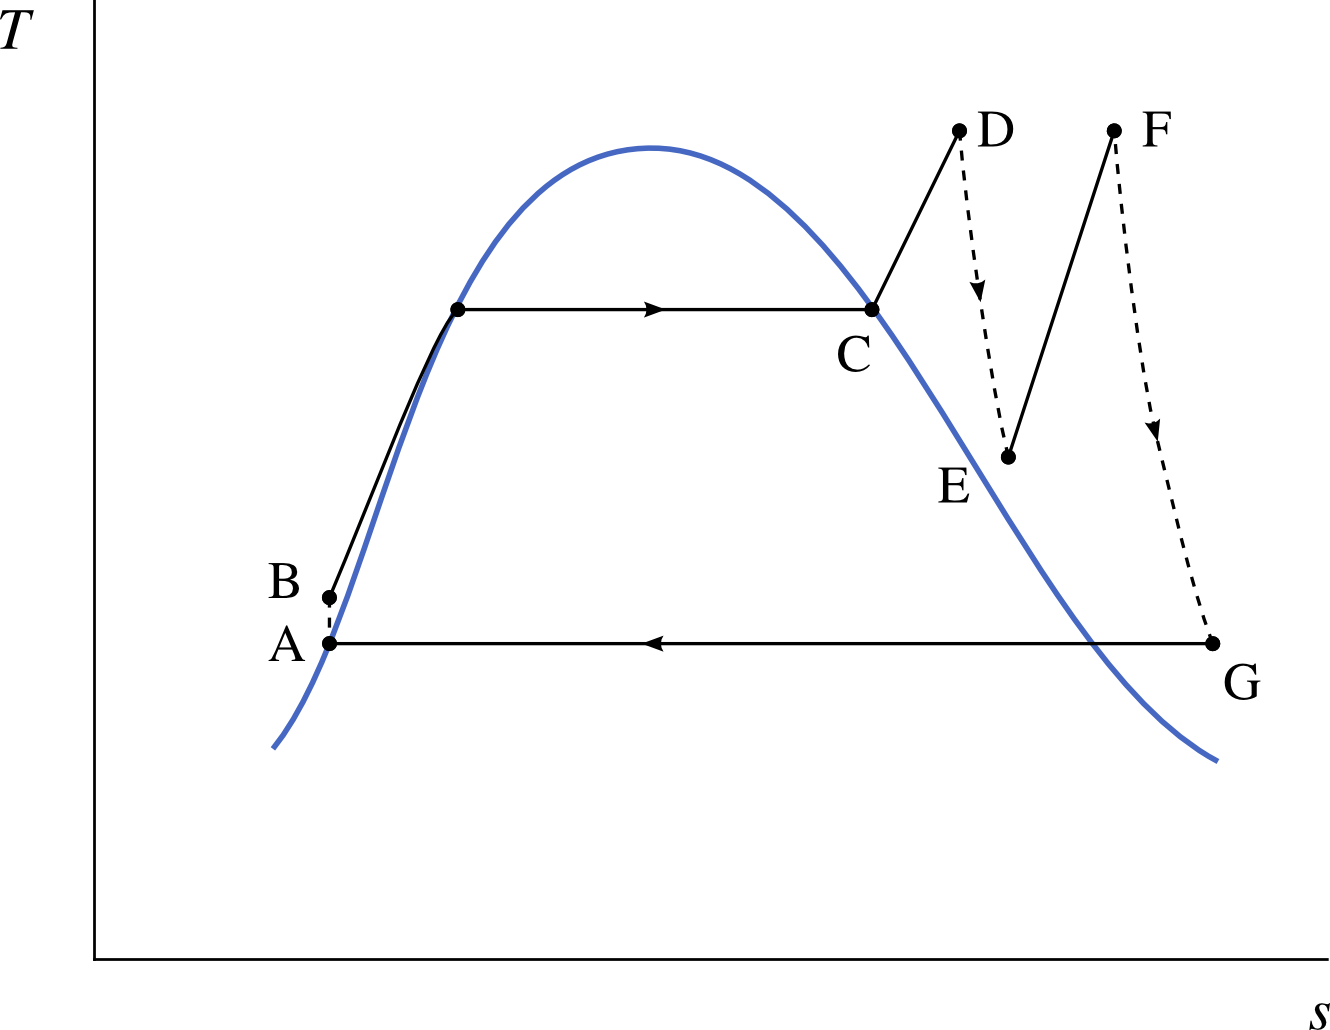
\includegraphics[width=10cm]{images/ts_lv_rankine_surchauffe_resurchauffe.png}
			\end{center}
			\supercaption{Diagramme température-entropie d’une centrale à vapeur fonctionnant sur un cycle de Rankine resurchauffé.}{schéma \cczero \oc}
			\label{fig_ts_lv_surchauffe_resurchauffe}
		\end{figure}

		Avec cette modification, la détente dans la turbine est interrompue ; et la vapeur est conduite dans une nouvelle série de tubes pour porter à nouveau sa température à haute température (usuellement aux limites métallurgiques de la turbine). La détente est alors complétée jusqu’à la pression du condenseur.

		Le rendement global de l’installation est augmenté si la température moyenne de chauffage l’est aussi ; il faut donc choisir avec soin la pression de la resurchauffe. La consommation spécifique, elle, est diminuée dans tous les cas, avec les avantages décrits plus haut.



	\subsection{La régénération}
	\label{ch_regeneration}

		Lorsque Rankine a modifié le cycle de Carnot, il a réduit le travail fourni pour compresser l’eau, et augmenté la chaleur nécessaire pour l’amener en entrée de turbine. En contrepartie, le rendement thermodynamique a diminué : en effet, lorsque l’eau pénètre dans la chaudière, sa température est faible. Elle reçoit de la chaleur de façon non-réversible.

		Pour augmenter la réversibilité du cycle (et donc son rendement), il est possible de réchauffer l’eau progressivement, en utilisant la chaleur en provenance de la turbine (où la température de la vapeur varie). Cette technique est nommée \vocab{régénération}. On peut ainsi imaginer un cycle comme décrit en figures~\ref{fig_circuit_regeneration} et~\ref{fig_ts_lv_regeneration} ci-dessous, où l’eau liquide en sortie de pompe est réchauffée progressivement en refroidissant la turbine.

		\begin{figure}
			\begin{center}
				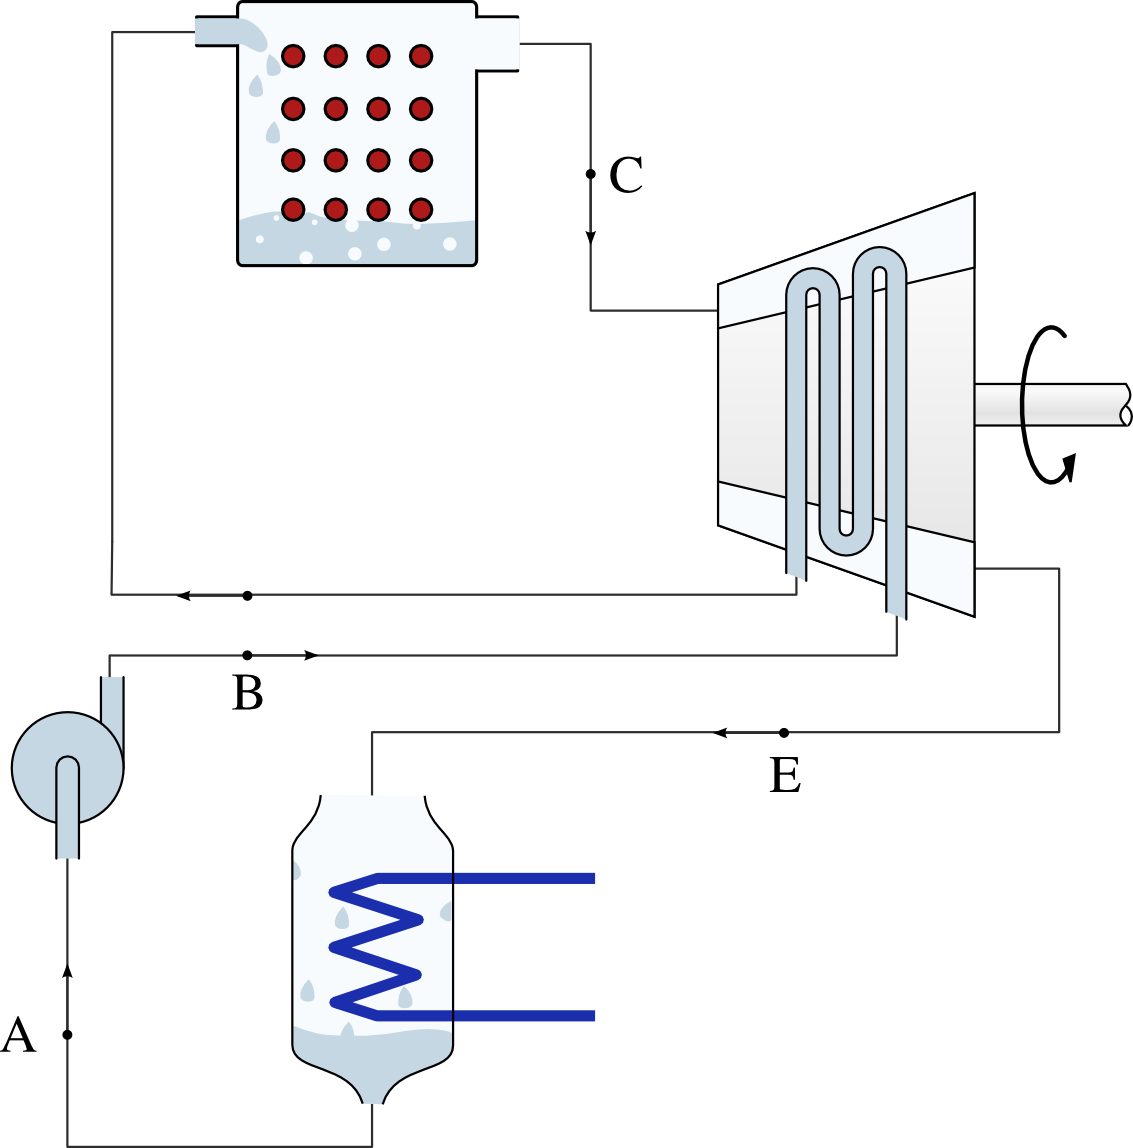
\includegraphics[height=11cm]{images/circuit_regeneration.png}
			\end{center}
			\caption{Circuit d’une centrale à vapeur avec régénération. On prélève de la chaleur à la turbine pour réchauffer l’eau liquide avant qu’elle ne pénètre dans la chaudière. Idéalement, l’échange de chaleur se fait de façon réversible.}
			\label{fig_circuit_regeneration}
		\end{figure}

		\begin{figure}
			\begin{center}
				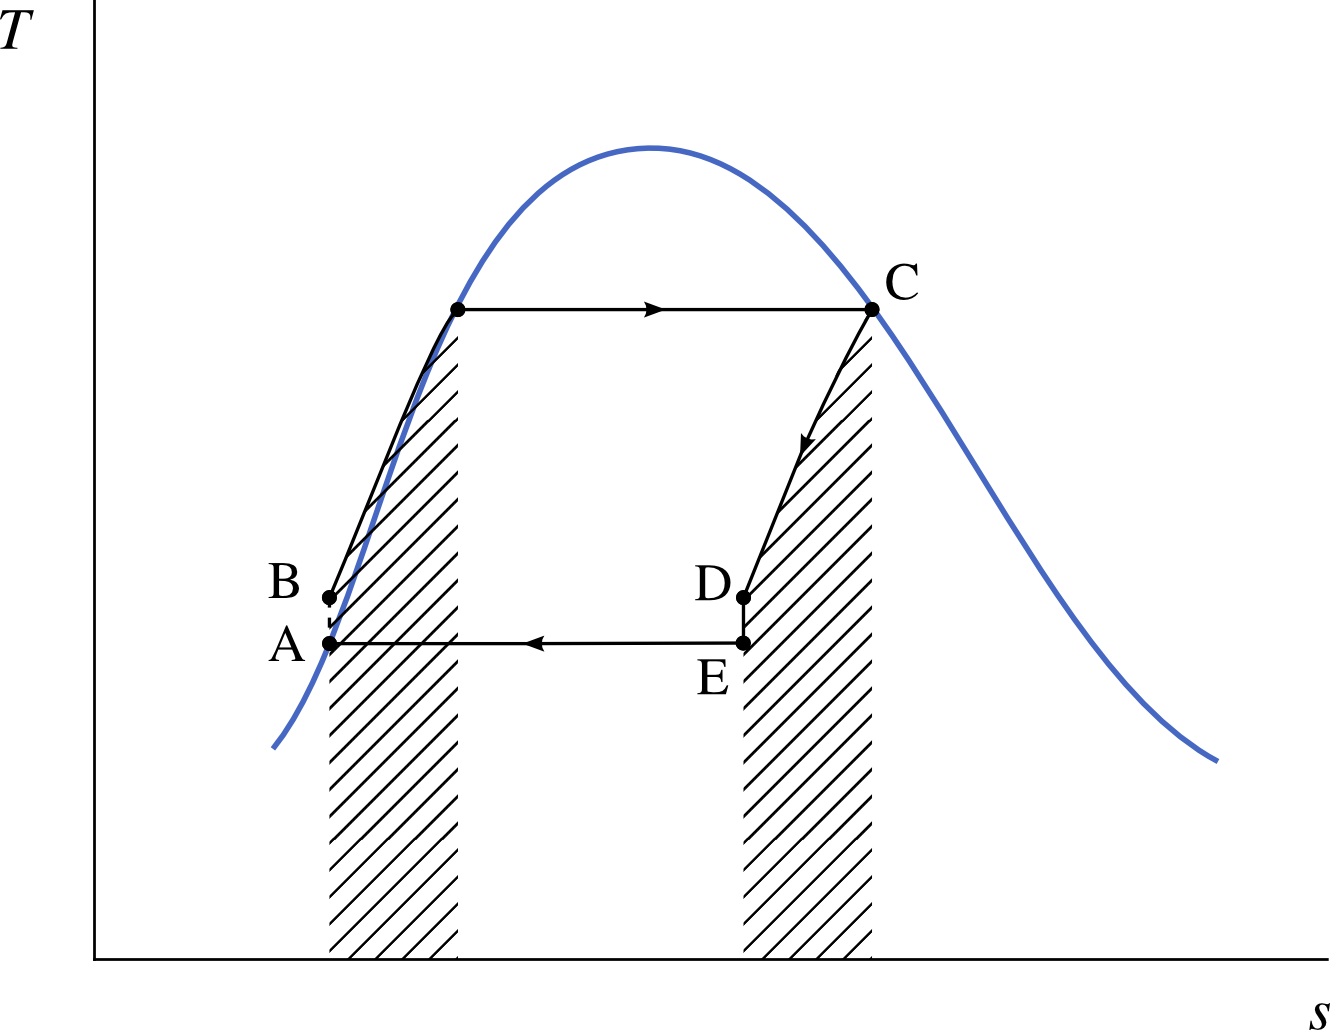
\includegraphics[width=10cm]{images/ts_lv_regeneration.png}
			\end{center}
			\caption{Diagramme température-entropie d’une centrale à vapeur avec régénération.}
			\label{fig_ts_lv_regeneration}
		\end{figure}


		Dans le cas limite où toute la chaleur utilisée lors de la régénération est transmise avec une différence de température infiniment faible, le cycle est réversible et le rendement du moteur de Carnot est atteint même si l’on ne suit pas à proprement parler le cycle de Carnot.

		En pratique hélas, un tel dispositif est difficile à réaliser. En effet, la transmission réversible de chaleur est complexe à mettre en place dans la turbine, élément dont la conception et la fabrication sont déjà très coûteuses. De plus, le refroidissement de la vapeur réduit son titre, augmentant la quantité d’eau liquide érodant les pièces de la turbine.

		Pour mettre en place la régénération, on a donc recours à la technique de \vocab{prélèvement turbine}. De la vapeur est ponctionnée depuis la turbine, et mélangée à l’eau liquide en sortie de pompe (figures~\ref{fig_cycle_prélèvement_vapeur} et~\ref{fig_ts_lv_prelevement_vapeur}). On obtient ainsi un transfert de chaleur qu’il est aisé de mettre en œuvre.

		\begin{figure}
			\begin{center}
				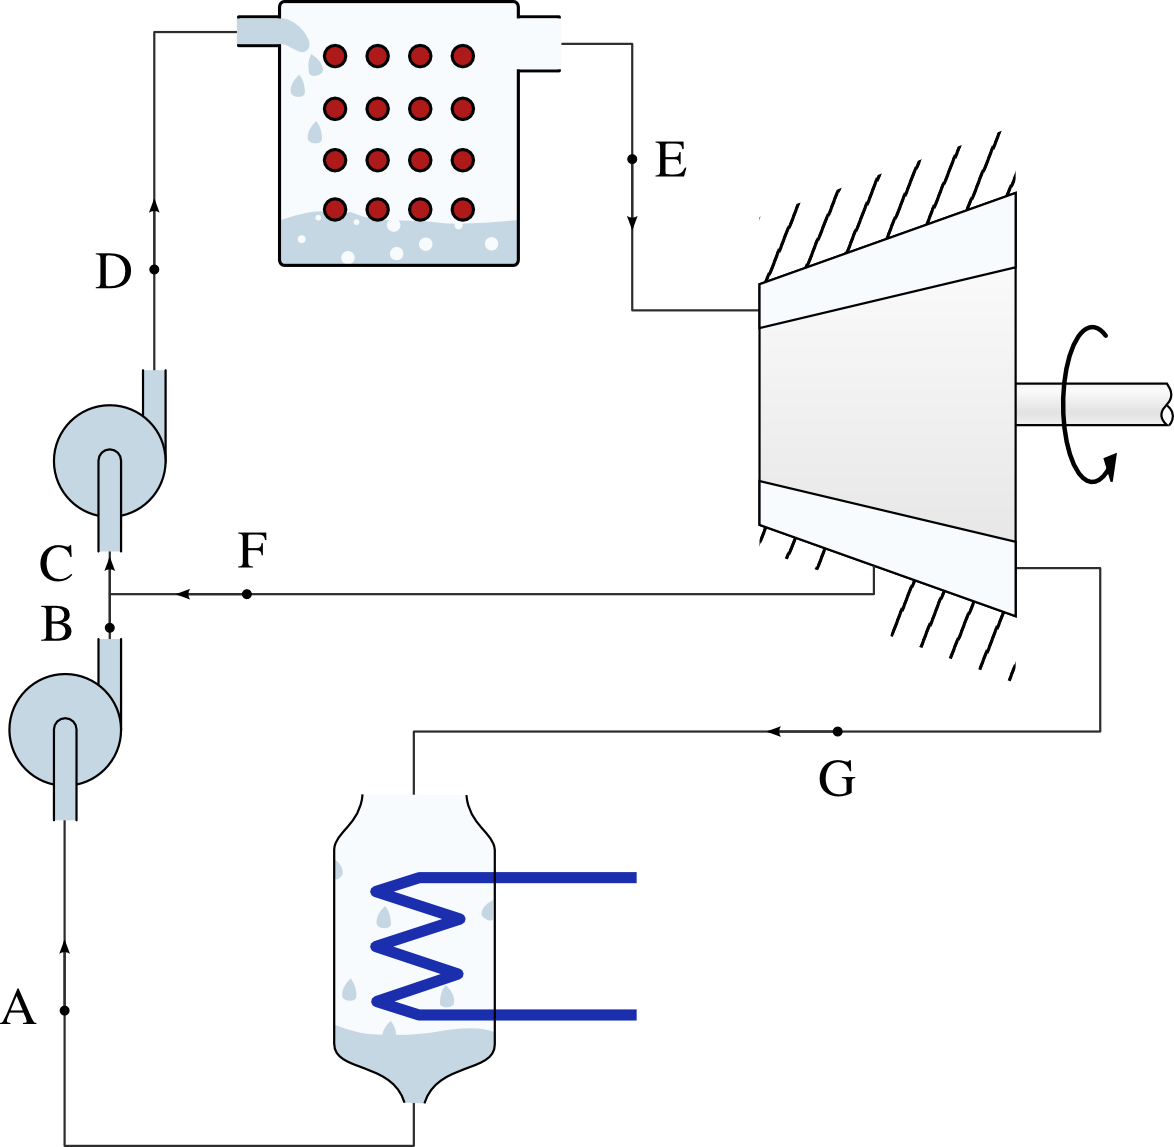
\includegraphics[height=11cm]{images/circuit_prelevement.png}
			\end{center}
			\supercaption{Circuit d’une centrale à vapeur avec prélèvement de vapeur. La vapeur extraite prématurément de la turbine est utilisée pour réchauffer l’eau liquide pendant le pompage.}{schéma \ccbysa \olivier}
			\label{fig_cycle_prélèvement_vapeur}
		\end{figure}

		\begin{figure}
			\begin{center}
				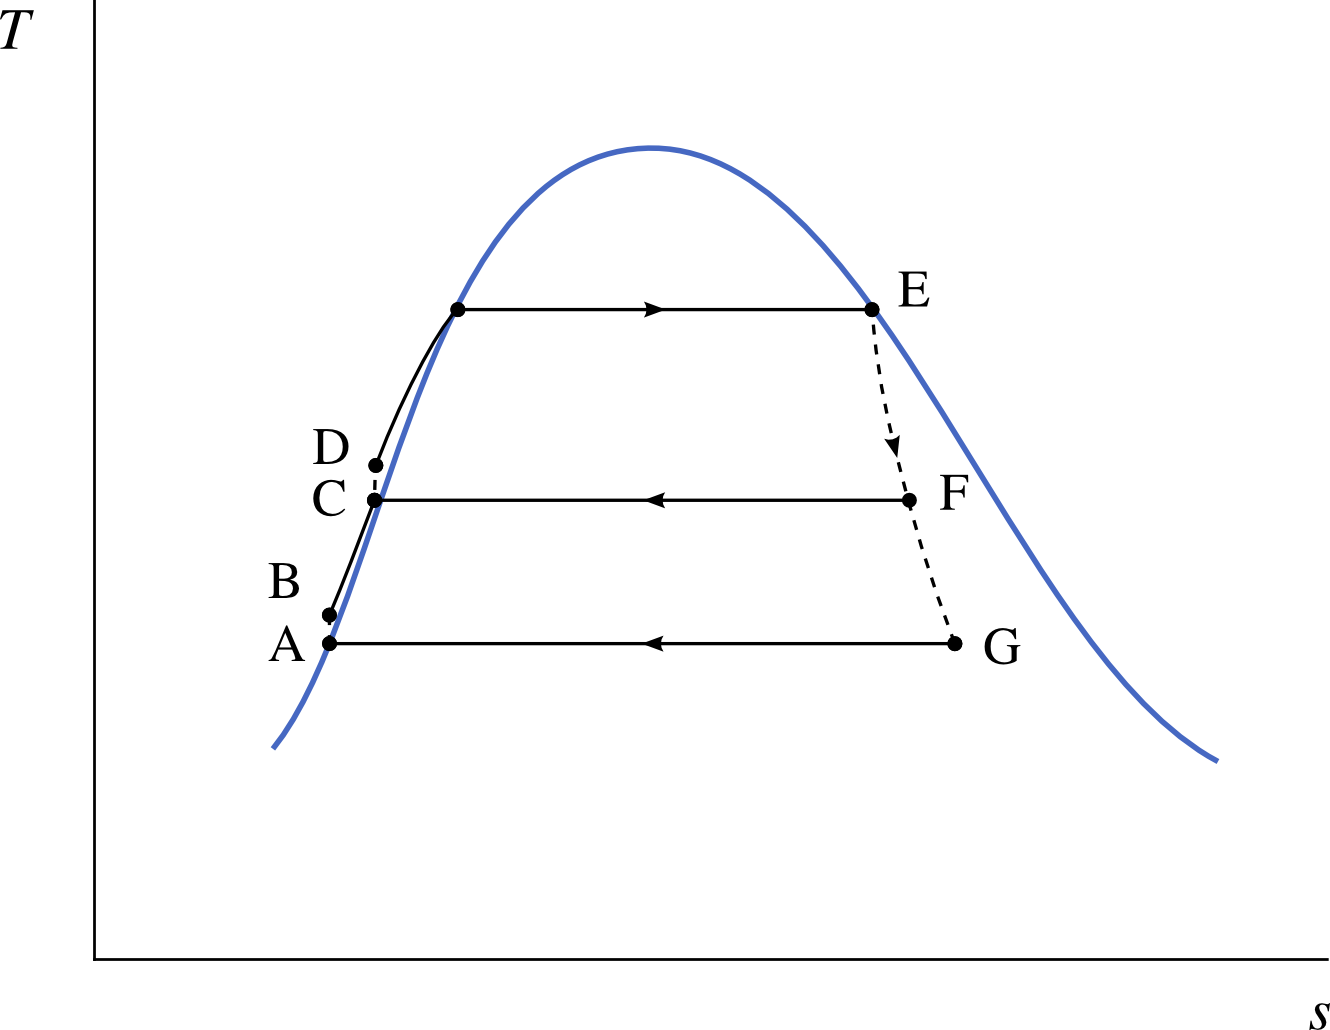
\includegraphics[width=10cm]{images/ts_lv_prelevement.png}
			\end{center}
			\supercaption{Diagramme température-entropie d’une centrale à vapeur avec prélèvement de vapeur.}{schéma \cczero \oc}
			\label{fig_ts_lv_prelevement_vapeur}
		\end{figure}

		En pratique, de nombreux prélèvements (judicieusement appelés \vocab{bleeds}, ou «~saignements~» en anglais) sont effectués dans les circuits de centrale à vapeur, pour contrôler les flux de chaleur (\cref{fig_grosse_centrale_vapeur}). Ils permettent accessoirement, par le biais de vannes de décharge, de réguler précisément les débits de masse et adapter ainsi rapidement la puissance de l’installation à la demande.

		\begin{landscape}
		\begin{figure}
		 	\begin{center}
		 			\vspace{-1.5cm}%handmade
				\centerline{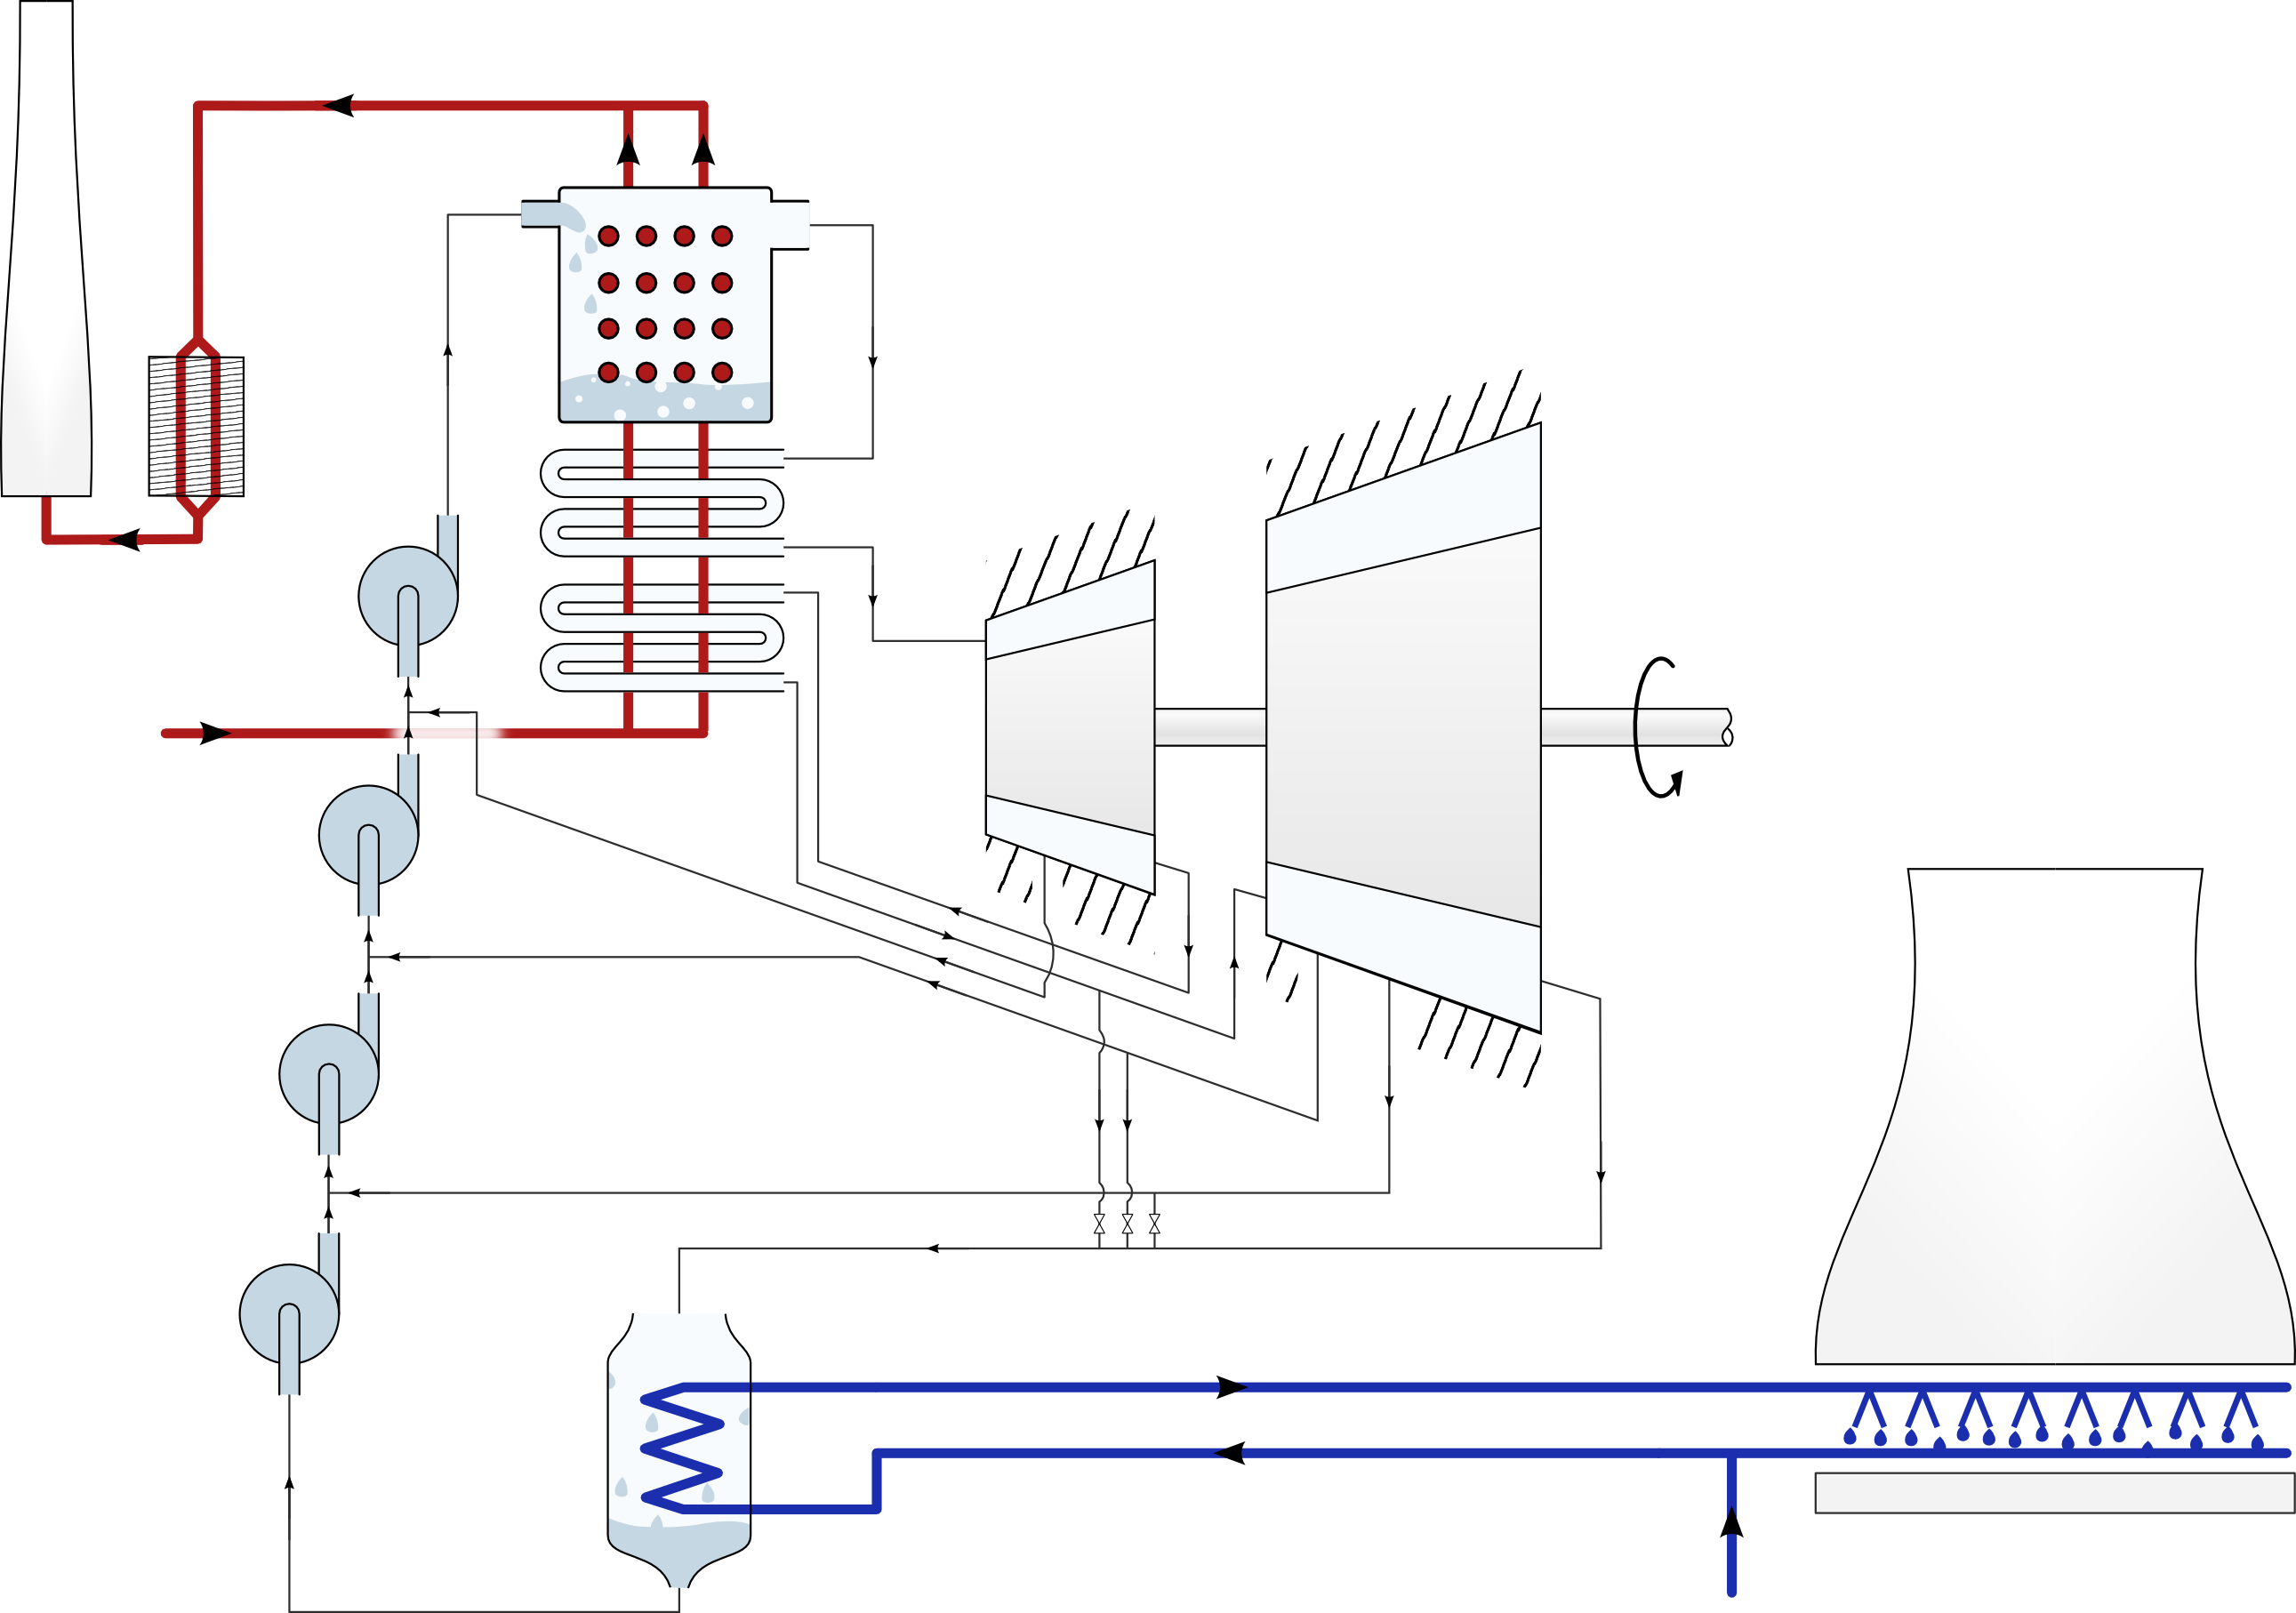
\includegraphics[width=20cm]{images/circuit_complet.png}}
			\end{center}
			\supercaption{Installation à vapeur mêlant surchauffe, resurchauffe, régénération, et conduits de décharge.
		Il est laissé à l’étudiant/e curieux/se le loisir de tracer les évolutions sur un diagramme température-entropie, et de s’imaginer aux commandes de l’installation alimentant sa cafetière en électricité.}{schéma \ccbysa \olivier}
			\label{fig_grosse_centrale_vapeur}
		\end{figure}
		\end{landscape}
